% ============================================================================
% Agentic Programming for Economic Research
% CES, LMU Munich, 18 November 2026 -- 150 minutes (2 x 70 min, 10-min break)
% Lineage: Geneva (May 2026) -> RWTH Aachen Session 9 (October 2026) -> this standalone lecture.
% Compile: latexmk -pdf Agentic_Programming_Munich.tex   (or: make)
% ============================================================================

\documentclass[aspectratio=169,10pt]{beamer}

% ---------- Theme and colors ----------
\usecolortheme{dove}
\setbeamertemplate{navigation symbols}{}
\setbeamertemplate{footline}{%
  \hfill\usebeamerfont{page number in head/foot}%
  \usebeamercolor[fg]{normal text}%
  \insertframenumber\,/\,\inserttotalframenumber\kern1em\vskip4pt}
\setbeamerfont{frametitle}{size=\Large}

% ---------- Packages ----------
\usepackage[utf8]{inputenc}
\usepackage[T1]{fontenc}
\usepackage{amsmath,amssymb,amsfonts}
\usepackage{bm}
\usepackage{graphicx}
\usepackage{tikz}
\usetikzlibrary{shapes,arrows.meta,positioning,calc,fit,backgrounds,
                 patterns,decorations.pathreplacing,shadows.blur}
\usepackage{booktabs}
\usepackage{hyperref}
\usepackage{multicol}
\usepackage{xcolor}
\usepackage{listings}
\usepackage{pifont}
\usepackage{colortbl}

% ---------- Custom colors ----------
\definecolor{uzhblue}{rgb}{0,0,0.5}
\definecolor{uzhgreylight}{RGB}{236,238,241}
\definecolor{uzhgreydark}{RGB}{81,86,94}
\definecolor{harvardcrimson}{RGB}{153,0,0}
\definecolor{unil@blue}{RGB}{0,140,204}
\definecolor{unil@black}{RGB}{35,31,32}
\definecolor{darkgreen}{RGB}{0,100,0}
\definecolor{darkred}{RGB}{139,0,0}
\definecolor{softblue}{RGB}{70,130,180}
\definecolor{softorange}{RGB}{230,159,0}
\definecolor{softgreen}{RGB}{0,158,115}
\definecolor{level0}{RGB}{200,200,200}
\definecolor{level1}{RGB}{180,200,220}
\definecolor{level2}{RGB}{140,180,220}
\definecolor{level3}{RGB}{100,160,220}
\definecolor{level4}{RGB}{60,130,200}
\definecolor{level5}{RGB}{30,90,160}

% ---------- Listings ----------
\lstset{
    language=Python,
    basicstyle=\small\ttfamily,
    keywordstyle=\color{uzhblue}\bfseries,
    commentstyle=\color{uzhgreydark}\itshape,
    stringstyle=\color{darkgreen},
    showstringspaces=false,
    breaklines=true,
    frame=none,
    xleftmargin=0pt,
    aboveskip=4pt,
    belowskip=4pt,
    escapeinside={(*@}{@*)},
}
\lstdefinestyle{bash}{
    language=bash,
    basicstyle=\small\ttfamily,
    keywordstyle=\color{uzhblue}\bfseries,
    commentstyle=\color{uzhgreydark}\itshape,
    stringstyle=\color{darkgreen},
    showstringspaces=false,
    breaklines=true, frame=none,
    xleftmargin=0pt, aboveskip=4pt, belowskip=4pt,
    morekeywords={claude,git,uv,npm,pip,cd,mkdir,ssh,squeue,sbatch,python3,pytest,latexmk,jq,cp},
}
\lstdefinestyle{prompt}{
    language={},
    basicstyle=\small\ttfamily,
    breaklines=true, frame=none,
    xleftmargin=6pt, aboveskip=4pt, belowskip=4pt,
    literate={>}{{\textcolor{harvardcrimson}{>}}}1,
}
% Plain text files shown verbatim: SKILL.md, agent files, CLAUDE.md, plans.
\lstdefinestyle{md}{
    language={},
    basicstyle=\tiny\ttfamily,
    breaklines=true, frame=single, rulecolor=\color{uzhgreydark!40},
    xleftmargin=2pt, aboveskip=2pt, belowskip=2pt,
    columns=fullflexible, keepspaces=true,
}
\lstdefinestyle{json}{
    language={},
    basicstyle=\tiny\ttfamily,
    breaklines=true, frame=single, rulecolor=\color{uzhgreydark!40},
    xleftmargin=2pt, aboveskip=2pt, belowskip=2pt,
    stringstyle=\color{darkgreen}, string=[b]",
    columns=fullflexible, keepspaces=true,
}

% ---------- Beamer colors ----------
\setbeamercolor{frametitle}{bg=uzhgreylight, fg=uzhblue}
\setbeamercolor{title}{fg=uzhblue}
\setbeamercolor{structure}{fg=uzhblue}
\setbeamercolor{block title}{bg=unil@blue, fg=white}
\setbeamercolor{block body}{bg=uzhgreylight}
\setbeamercolor{block title alerted}{bg=darkred,fg=white}
\setbeamercolor{block body alerted}{bg=red!5}
\setbeamercolor{block title example}{bg=darkgreen,fg=white}
\setbeamercolor{block body example}{bg=green!5}
\setbeamercolor{item}{fg=unil@black}
\setbeamercolor{normal text}{fg=unil@black}

% ---------- Commands ----------
\newcommand{\emphc}[1]{\textcolor{harvardcrimson}{#1}}
\hypersetup{colorlinks,linkcolor=harvardcrimson,urlcolor=harvardcrimson}
\newcommand{\R}{\mathbb{R}}
\newcommand{\livedemo}{%
  \tikz[baseline=(X.base)]{\node[fill=harvardcrimson,text=white,
  rounded corners=2pt,inner sep=3pt,font=\scriptsize\bfseries](X){LIVE DEMO};}}
\newcommand{\walkthrough}{%
  \tikz[baseline=(X.base)]{\node[fill=level4,text=white,
  rounded corners=2pt,inner sep=3pt,font=\scriptsize\bfseries](X){WALK-THROUGH};}}
\newcommand{\boristip}[1]{%
  \tikz[baseline=(X.base)]{\node[fill=level4,text=white,
  rounded corners=2pt,inner sep=2pt,font=\tiny\bfseries](X){TIP #1};}}
% \stepmarker{n}: the seven-step ladder of the lead example with step n highlighted.
\newcommand{\stepmarker}[1]{%
  \tikz[baseline=-0.6ex]{\foreach \i in {1,...,7}{%
    \ifnum\i=#1 \node[fill=harvardcrimson,text=white,font=\tiny\bfseries,inner sep=2.5pt,minimum width=1.1em] at (\i*0.46,0) {\i};%
    \else \node[fill=uzhgreylight,text=uzhgreydark,font=\tiny,inner sep=2.5pt,minimum width=1.1em] at (\i*0.46,0) {\i};\fi}}%
  {\scriptsize\textcolor{uzhgreydark}{~Step #1}}}
% \chip{n}{text}: a numbered pill, used for the demo row on the plan slide.
\newcommand{\chip}[2]{\tikz[baseline=(X.base)]{\node[fill=uzhgreylight,rounded corners=3pt,inner sep=4pt,font=\small](X){\textcolor{harvardcrimson}{\textbf{#1}}~#2};}}
% \filebox{path}: the repository location of what the frame shows.
\newcommand{\filebox}[1]{%
  \vspace{0.2em}\par\noindent
  \colorbox{uzhgreylight}{\parbox{\dimexpr\textwidth-2\fboxsep\relax}{%
    \raggedright\scriptsize\textcolor{uzhgreydark}{\textbf{In the repo:}} \texttt{#1}}}}
\newcommand{\partcard}[2]{%
  \begin{frame}{}\vfill\begin{center}
  {\Huge \textcolor{uzhblue}{\textbf{Part #1}}}\\[12pt]{\LARGE #2}
  \end{center}\vfill\end{frame}}

% ---------- TikZ styles ----------
\tikzset{
    cbox/.style={draw, rounded corners=4pt, minimum height=1.2cm,
                 minimum width=2.6cm, align=center, font=\small,
                 fill=#1, text=white},
    phase/.style={draw, rounded corners=3pt, fill=#1,
                  minimum width=4cm, minimum height=0.7cm,
                  font=\scriptsize, align=center},
    spoke/.style={draw, rounded corners=3pt, fill=#1,
                  minimum width=1.6cm, minimum height=0.55cm,
                  font=\tiny, text=white, align=center},
    fblock/.style={draw, rounded corners=5pt, fill=#1,
                   minimum width=2.6cm, minimum height=0.8cm,
                   font=\small, text=white, align=center},
    pipestep/.style={draw, rounded corners=3pt, fill=#1,
                     minimum width=2.6cm, minimum height=0.55cm,
                     font=\tiny, text=white, align=center},
    tpane/.style={draw, rounded corners=2pt, fill=#1,
                  minimum width=2.6cm, minimum height=1cm,
                  font=\tiny, align=center},
}

% ---------- Title ----------
\title[Agentic programming -- CES Munich 2026]%
{Agentic Programming for Economic Research}
\subtitle{AI coding agents in the research workflow: from prompt to verified result}
\author{Simon Scheidegger}
\institute[HEC Lausanne \& LSE]{HEC, University of Lausanne\\Grantham Research Institute, London School of Economics}
\date{Lecture at the Center for Economic Studies (CES), LMU Munich\\18 November 2026}

\begin{document}

% ============================================================================
% TITLE & INTRO
% ============================================================================

{\setbeamercolor{background canvas}{bg=uzhgreylight}
\begin{frame}
\titlepage
\vspace{-0.2cm}
\begin{center}
{\footnotesize Slides, code and every file shown today: \url{https://github.com/sischei/agentic_programming_munich_1126}}
\end{center}
\vfill
{\tiny\textcolor{uzhgreydark}{The lecture draws on Korinek (2023, \emph{JEL}); Schluntz \& Zhang (2024); Cherny (2025); Bilionis et al.\ (2026); Goldsmith-Pinkham (2026); and the Claude Code documentation (November 2026).}}
\end{frame}
}

% --- Contents ---
\begin{frame}{Contents}
\vspace{0.3em}
\small
\renewcommand{\arraystretch}{1.15}
\begin{tabular}{@{}p{1.1cm} p{8.4cm} r@{}}
\multicolumn{3}{@{}l}{\textbf{Block 1 (70 min): working with the agent}} \\
\textbf{I} & Orientation \& mental models; the running example & 5 \\
\textbf{II} & Setting up: Claude Code, git, the demo project & 13 \\
\textbf{III} & The core interaction loop; a task in plan mode & 20 \\
\textbf{IV} & Prompt engineering for research & 28 \\
 & \emph{Break, 10 minutes} & 35 \\[4pt]
\multicolumn{3}{@{}l}{\textbf{Block 2 (70 min): extending and trusting the agent}} \\
\textbf{V} & Project memory: \texttt{CLAUDE.md} & 36 \\
\textbf{VI} & Skills, subagents, hooks, MCP & 39 \\
\textbf{VII} & Autonomous loops: \texttt{/goal} & 46 \\
\textbf{VIII} & From plan to table and figure & 57 \\
\textbf{IX} & Verification, reproducibility, governance & 63 \\
 & Wrap-up: quick reference, takeaways, conclusion & 70 \\
\end{tabular}

\vspace{0.6em}
{\footnotesize One example throughout: a neural solver for a growth model, built with the agent in seven steps (slide 12). Live demos in Parts II, III, VI, VII and VIII.}
\end{frame}

% --- Why now, what it is ---
\begin{frame}{Why Now, and What ``Agentic'' Means}
\begin{columns}[T]
\column{0.50\textwidth}
\textbf{The bottleneck has shifted.}
\begin{itemize}\itemsep3pt
  \item Old: can you \emph{write} the code?
  \item New: can you \emphc{specify} what you want, and \emphc{verify} what you get?
\end{itemize}
\vspace{0.4em}
Both reward domain expertise: which question, which moment, which residual must be zero. That is the economist's job, and now the whole job.

\vspace{0.7em}
\begin{block}{Agentic programming}
An AI system that reads your project, edits code, runs it, inspects the output and iterates towards a goal. Not autocomplete, not a chat window, not an autopilot for judgement.
\end{block}

\column{0.46\textwidth}
\begin{center}
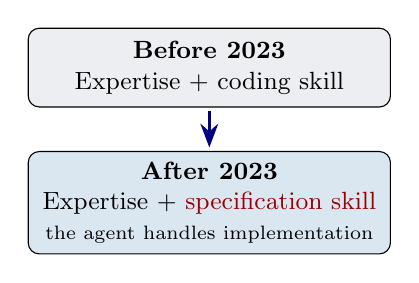
\begin{tikzpicture}[scale=0.78, every node/.style={font=\small}]
    \node[draw, rounded corners, fill=uzhgreylight, minimum width=4.6cm,
          minimum height=1cm, align=center] at (0,3.6)
          {\textbf{Before 2023}\\Expertise + coding skill};
    \draw[-{Stealth[length=3mm]}, very thick, uzhblue] (0,2.9) -- (0,2.3);
    \node[draw, rounded corners, fill=softblue!20, minimum width=4.6cm,
          minimum height=1.3cm, align=center] at (0,1.4)
          {\textbf{After 2023}\\Expertise + \emphc{specification skill}\\{\scriptsize the agent handles implementation}};
\end{tikzpicture}
\end{center}
\vspace{0.2em}
\textbf{Two traps}
\begin{itemize}\itemsep3pt
  \item \textcolor{darkred}{\textbf{Hype.}} Self-assessed speed-ups are not evidence: METR (2025) found experienced developers 19\,\% \emph{slower} while believing they were faster.
  \item \textcolor{darkred}{\textbf{Dismissal.}} ``Just autocomplete.'' Agents plan, run, debug and iterate for hours.
\end{itemize}
\end{columns}
\end{frame}

% --- Today's plan ---
\begin{frame}{Today: Two Blocks, Five Live Demos, One Solver}
\begin{columns}[T]
\column{0.49\textwidth}
\begin{block}{Block 1 (70 min): work with the agent}
\begin{itemize}\itemsep2pt
  \item What an agent is, and what it is not
  \item Setting up: Claude Code, git, the demo project
  \item Steering it: the feedback loop, plan mode
  \item Writing a research prompt that works
\end{itemize}
\end{block}
\column{0.49\textwidth}
\begin{block}{Block 2 (70 min): extend and trust it}
\begin{itemize}\itemsep2pt
  \item Project memory: \texttt{CLAUDE.md}
  \item Skills, subagents, hooks, MCP
  \item Autonomous loops: \texttt{/goal}
  \item Verification, disclosure, governance
\end{itemize}
\end{block}
\end{columns}

\vspace{0.4em}
\textbf{One example throughout:} a neural solver for a growth model, built with the agent in seven steps, each checked against a known answer.

\vspace{0.4em}
\textbf{Five live demos}\par\vspace{0.25em}
\chip{1}{build the project}\;
\chip{2}{Step 1 in plan mode}\;
\chip{3}{a skill, then a subagent}\;
\chip{4}{\texttt{/goal} against five tests}\;
\chip{5}{prompt $\to$ table + figure}

\vspace{0.45em}
\textbf{You leave with} a verified solver, a prompt discipline, and a repository that replays everything at home. {\scriptsize\textcolor{uzhgreydark}{Nothing to install today. The TIP badges point to Boris Cherny's ten tips, collected in the wrap-up.}}
\end{frame}

% ============================================================================
% PART I: ORIENTATION & MENTAL MODELS
% ============================================================================
\partcard{I}{Orientation \& Mental Models}

% --- Chatbox vs agentic + hierarchy ---
\begin{frame}{From Chatbox to Agent: Tiers of Tooling}
\begin{alertblock}{Paul Goldsmith-Pinkham (2026)}
\itshape ``Web-based AI is like exchanging emails with a smart person.
Claude Code is like having them sit next to you, coding while you talk.''
\end{alertblock}

\vspace{0.4em}
\begin{center}
\small
\renewcommand{\arraystretch}{1.25}
\begin{tabular}{c p{6.4cm} p{5.2cm}}
\toprule
\textbf{Tier} & \textbf{Capability} & \textbf{Examples (November 2026)} \\
\midrule
\textbf{0--1} & Browser chatbot; the task lives in your head & ChatGPT, Claude.ai, Gemini \\
\textbf{2} & Inline IDE assistant: edits the file you have open & Copilot, Cursor \\
\rowcolor{softblue!10}
\textbf{3} & \textbf{Terminal agent}: reads and writes files, runs code, uses git & \textbf{Claude Code}, Codex CLI, Gemini CLI \\
\rowcolor{softblue!10}
\textbf{4} & + external tools via MCP (Model Context Protocol) & + Zotero, GitHub, databases, HPC \\
\textbf{5} & Closed-loop autonomy with a verifier & \texttt{/goal}, headless (batch) runs \\
\bottomrule
\end{tabular}
\end{center}

\vspace{0.3em}
\textbf{Same models, different scaffolding.} From Tier 3 on, the agent \emph{does} the work: a fast junior research assistant who never tires and never asks whether a result makes economic sense. Today: Tiers 3--4, with a taste of 5.
\end{frame}

% --- Context Window ---
\begin{frame}[fragile]{The Context Window, the Most Important Mental Model}
A language model has \emphc{no persistent memory}: every turn, the whole conversation so far is sent to it as one document, the \emphc{context window}.

\vspace{0.2em}
\begin{center}
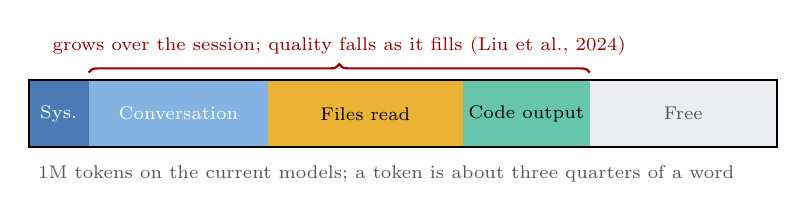
\begin{tikzpicture}[scale=0.95, transform shape]
    \def\barwidth{10}
    \def\barheight{0.9}
    \fill[level5!80] (0,0) rectangle (0.8,\barheight);
    \node[font=\scriptsize, text=white] at (0.4,0.45) {Sys.};
    \fill[level3!80] (0.8,0) rectangle (3.2,\barheight);
    \node[font=\scriptsize, text=white] at (2.0,0.45) {Conversation};
    \fill[softorange!80] (3.2,0) rectangle (5.8,\barheight);
    \node[font=\scriptsize] at (4.5,0.45) {Files read};
    \fill[softgreen!60] (5.8,0) rectangle (7.5,\barheight);
    \node[font=\scriptsize] at (6.65,0.45) {Code output};
    \fill[uzhgreylight] (7.5,0) rectangle (\barwidth,\barheight);
    \node[font=\scriptsize, text=uzhgreydark] at (8.75,0.45) {Free};
    \draw[thick] (0,0) rectangle (\barwidth,\barheight);
    \node[font=\scriptsize, anchor=west, text=uzhgreydark] at (0,-0.35) {1M tokens on the current models; a token is about three quarters of a word};
    \draw[decorate, decoration={brace, amplitude=3pt}, thick, harvardcrimson]
        (0.8,\barheight+0.1) -- (7.5,\barheight+0.1)
        node[midway, above=3pt, font=\scriptsize, text=harvardcrimson] {grows over the session; quality falls as it fills (Liu et al., 2024)};
\end{tikzpicture}
\end{center}

\vspace{0.1em}
\begin{columns}[T]
\column{0.48\textwidth}
\textbf{What Claude Code does about it}
\begin{itemize}\itemsep2pt
  \item \texttt{/context}: what is loaded right now
  \item \texttt{/compact}: summarise, reload \texttt{CLAUDE.md} (the project memory, Part V)
  \item Subagents (Part VI): their own window
\end{itemize}
\column{0.48\textwidth}
\textbf{What you do about it}
\begin{itemize}\itemsep2pt
  \item \texttt{/clear} between unrelated tasks
  \item Write state to disk, not into the conversation
  \item \texttt{/compact} at about 60\,\% used
\end{itemize}
\end{columns}

\vspace{0.2em}
\begin{alertblock}{The \#1 failure pattern: kitchen-sink sessions}
Unrelated tasks in one session: each adds context that degrades all the others.
\end{alertblock}
\end{frame}

% --- Task Taxonomy ---
\begin{frame}{Where the Agent Excels, and Where It Struggles}
\begin{center}
\small
\renewcommand{\arraystretch}{1.0}
\begin{tabular}{p{6.0cm} c p{5.2cm}}
\toprule
\textbf{Task type} & \textbf{Quality} & \textbf{Notes} \\
\midrule
Data cleaning, reshaping, merging & \textcolor{darkgreen}{\textbf{Excellent}} & Fastest return on effort \\
Standard econometrics (OLS, IV, panel, GMM) & \textcolor{darkgreen}{\textbf{Excellent}} & Verify clustering, edge cases \\
Debugging cryptic errors & \textcolor{darkgreen}{\textbf{Excellent}} & Faster than any forum \\
Porting a notebook into a tested script & \textcolor{darkgreen}{\textbf{Excellent}} & Step 1 today \\
\midrule
Methods outside its training data & \textcolor{softorange}{\textbf{Moderate}} & Needs your guidance \\
Numerical choices: grids, weights, tolerances & \textcolor{softorange}{\textbf{Moderate}} & Runs cleanly either way \\
\midrule
Novel theory derivation & \textcolor{darkred}{\textbf{Poor}} & Never without a computational check \\
``Small residual, wrong answer'': method or code? & \textcolor{darkred}{\textbf{Poor}} & You decide \\
Verifying its own work & \textcolor{darkred}{\textbf{Poor}} & \emphc{Never skip human review} \\
\bottomrule
\end{tabular}
\end{center}

\vspace{0.2em}
\begin{alertblock}{Bilionis et al.\ (2026) and Hans \& Bilionis (2026), after giving papers to an agent to replicate}
A \emphc{very fast second-year PhD student}: excellent at known methods, mediocre at novel ones.
\end{alertblock}
\end{frame}

% --- Master workflow ---
\begin{frame}{The Workflow: Explore $\to$ Plan $\to$ Implement $\to$ Commit}
Four phases, from the Claude Code team, for every non-trivial task.

\vspace{0.5em}
\begin{center}
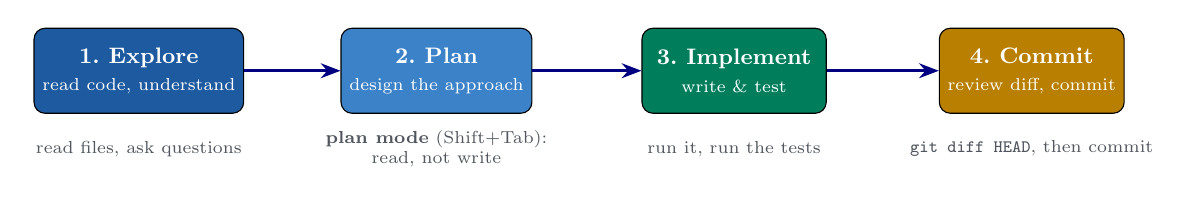
\begin{tikzpicture}[
    arr/.style={-{Stealth[length=2.5mm]}, very thick, uzhblue},
    scale=0.9, transform shape
]
    \node[cbox=level5] (explore) at (0,0) {\textbf{1.\ Explore}\\{\scriptsize read code, understand}};
    \node[cbox=level4] (plan) at (4.2,0) {\textbf{2.\ Plan}\\{\scriptsize design the approach}};
    \node[cbox=softgreen!80!black] (impl) at (8.4,0) {\textbf{3.\ Implement}\\{\scriptsize write \& test}};
    \node[cbox=softorange!80!black] (commit) at (12.6,0) {\textbf{4.\ Commit}\\{\scriptsize review diff, commit}};
    \draw[arr] (explore) -- (plan);
    \draw[arr] (plan) -- (impl);
    \draw[arr] (impl) -- (commit);
    \node[font=\scriptsize, text=uzhgreydark, align=center] at (0,-1.1)
        {read files, ask questions};
    \node[font=\scriptsize, text=uzhgreydark, align=center] at (4.2,-1.1)
        {\textbf{plan mode} (Shift+Tab):\\read, not write};
    \node[font=\scriptsize, text=uzhgreydark, align=center] at (8.4,-1.1)
        {run it, run the tests};
    \node[font=\scriptsize, text=uzhgreydark, align=center] at (12.6,-1.1)
        {\texttt{git diff HEAD}, then commit};
\end{tikzpicture}
\end{center}

\vspace{0.6em}
\begin{columns}[T]
\column{0.50\textwidth}
\boristip{2} \textbf{Pour energy into the plan}, so the agent implements in one pass. If it goes sideways, go \emph{back} to plan mode instead of pushing through.

\vspace{0.4em}
\textbf{Plan mode} is a permission mode: the agent reads and thinks, then writes a plan you approve, edit or reject. Nothing on disk changes until you say so.
\column{0.46\textwidth}
\textbf{Skip planning only for} one-line fixes and tasks you have specified in full.

\vspace{0.4em}
\textbf{Always plan for} anything touching more than two files, any change to an estimation or a loss, anything that goes into a paper.
\end{columns}
\end{frame}

% --- The running example ---
\begin{frame}{The Running Example: A Growth Model}
\small
Everything today happens on the stochastic Brock--Mirman growth model:
\begin{align*}
Y_t &= z_t K_t^{\alpha}, \qquad C_t = (1 - s_t)\, Y_t,\\
K_{t+1} &= (1-\delta) K_t + s_t Y_t, \qquad \log z_{t+1} = \varrho \log z_t + \sigma \varepsilon_{t+1}, \quad \varepsilon \sim N(0,1),
\end{align*}
log utility, $\alpha = 0.36$, $\delta = 0.10$, $\sigma = 0.04$, $\beta = 0.96$, $\varrho = 0.9$. The household chooses the savings rate $s_t$.

\vspace{0.3em}
\begin{block}{The equilibrium condition, and the number every check today looks at}
The Euler equation, $1/C_t = \beta\,\mathbb{E}_t\!\left[(1-\delta+\alpha z_{t+1}K_{t+1}^{\alpha-1})/C_{t+1}\right]$. Its \emphc{residual} $r = \beta C\,\mathbb{E}[\,\cdot\,] - 1$, a fraction of consumption, is zero at the solution. Every check today asks how far from zero it is, and \emph{where}.
\end{block}

\vspace{0.3em}
\textbf{The lead example.} A \emphc{deep equilibrium net} (DEQN; Azinovic, Gaegauf and Scheidegger, 2022): a small neural network $s_\theta(z, K)$ for the savings rate, trained by gradient descent until the Euler equation holds on sampled states. Built \emph{with the agent} in seven steps, each graded against a known answer.
\filebox{code/brock\_mirman\_reference.py (167 lines), code/data/, code/deqn/README.md (every step, script and number)}
\end{frame}

\begin{frame}{The Running Example: Three Known Answers}
\small
\begin{columns}[T]
\column{0.31\textwidth}
\begin{block}{1. The closed form}
Step 1 uses the course notebook's calibration, $\delta = 1$ and $\beta = 0.99$: then the savings rate is the constant $s^* = \alpha\beta = 0.3564$.
\end{block}
\column{0.31\textwidth}
\begin{block}{2. The reference solver}
A conventional grid-based solver shipped with the repository: the policy for any $(\beta, \varrho)$ in two seconds, Euler errors $10^{-9}$. Steps 2--7.
\end{block}
\column{0.31\textwidth}
\begin{block}{3. The truth file}
Five simulated economies with hidden $\varrho$; the file is read once, at the end of Step 7.
\end{block}
\end{columns}

\vspace{0.6em}
\textbf{Why three.} The closed form grades the port; the solver grades the stochastic model, where no closed form exists; the truth file grades the estimation at the very end. An agent that must pass all three cannot talk its way through.

\vspace{0.6em}
\begin{alertblock}{The pattern to take home}
Build the twin with a known answer before you let an agent loose on your real problem. It is the cheapest verifier you will ever own.
\end{alertblock}
\end{frame}

\begin{frame}{The Seven Steps of the Lead Example}
\vspace{0.3em}
\begin{center}
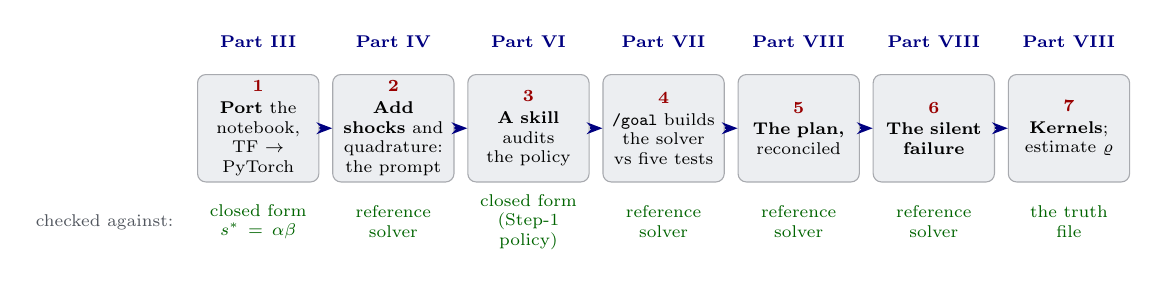
\begin{tikzpicture}[
  stepbox/.style={draw=uzhgreydark!50, fill=uzhgreylight, rounded corners=3pt, minimum width=1.75cm, minimum height=1.55cm, align=center, font=\scriptsize, text width=1.6cm, inner sep=2pt},
  truth/.style={font=\scriptsize, align=center, text width=1.75cm},
  part/.style={font=\scriptsize\bfseries, text=uzhblue},
  arr/.style={-{Stealth[length=2mm]}, thick, uzhblue}, scale=0.88, transform shape]
  \foreach \i/\p/\name in {
     1/III/{\textbf{Port} the notebook, TF $\to$ PyTorch},
     2/IV/{\textbf{Add shocks} and quadrature: the prompt},
     3/VI/{\textbf{A skill} audits the policy},
     4/VII/{\texttt{/goal} builds the solver vs five tests},
     5/VIII/{\textbf{The plan,} reconciled},
     6/VIII/{\textbf{The silent failure}},
     7/VIII/{\textbf{Kernels}; estimate $\varrho$}}{
     \node[part] at (\i*1.95-1.95, 1.25) {Part \p};
     \node[stepbox] (s\i) at (\i*1.95-1.95, 0) {\textcolor{harvardcrimson}{\textbf{\i}}\\[1pt]\name};
  }
  \foreach \i in {1,...,6}{\pgfmathtruncatemacro{\j}{\i+1}\draw[arr] (s\i) -- (s\j);}
  \foreach \i/\t in {1/{closed form\\$s^*=\alpha\beta$},2/{reference\\solver},3/{closed form\\(Step-1 policy)},4/{reference\\solver},5/{reference\\solver},6/{reference\\solver},7/{the truth\\file}}{
     \node[truth, text=darkgreen] at (\i*1.95-1.95, -1.35) {\t};
  }
  \node[font=\scriptsize, text=uzhgreydark, anchor=east] at (-1.1, -1.35) {checked against:};
\end{tikzpicture}
\end{center}

\vspace{0.6em}
\begin{columns}[T]
\column{0.48\textwidth}
\textbf{Each step introduces one tool:} 1 plan mode; 2 the six-component prompt; 3 a skill and a subagent; 4 \texttt{/goal} against five tests; 5 the plan, reconciled with the run; 6 the on-path check that catches a silent failure; 7 one prompt $\to$ table + figure.
\column{0.48\textwidth}
\textbf{Each step is graded:} by the closed form (Steps 1 and 3), by the reference solver (2, 4--7), by the truth file (7). The marker \stepmarker{3} on a slide says where we are.
\end{columns}
\filebox{code/deqn/ (scripts, tests, outputs); code/prompts.md (every prompt, in order)}
\end{frame}

% ============================================================================
% PART II: SETTING UP
% ============================================================================
\partcard{II}{Setting Up: Claude Code, Git, the Demo Project}

% --- Core Stack ---
\begin{frame}[fragile]{The Stack~\livedemo}
Four things: a terminal (or an IDE, or the desktop app), Claude Code, version control, Python.

\vspace{0.3em}
\begin{exampleblock}{Install (macOS / Linux / Windows), then check}
\begin{lstlisting}[style=bash, basicstyle=\scriptsize\ttfamily]
curl -fsSL https://claude.ai/install.sh | bash   # or brew / winget
claude --version && claude doctor                # then /login
\end{lstlisting}
\end{exampleblock}

\vspace{0.3em}
\begin{columns}[T]
\column{0.50\textwidth}
\boristip{7} \textbf{Where it runs}
\begin{itemize}\itemsep3pt
  \item Terminal: \texttt{claude} inside the project folder (today)
  \item VS Code and JetBrains: the same agent, diffs in the editor
  \item Desktop app and \texttt{claude.ai/code}: cloud sessions; your repository is copied to the vendor (Part IX)
\end{itemize}
\column{0.46\textwidth}
\begin{alertblock}{Privacy, first thing}
Anything the agent \emph{reads} is sent to the API. Deny rules (what it may not read) and hooks (what it may not do), Part VI, keep sensitive paths out; retention and training defaults differ by plan.
\end{alertblock}
\end{columns}
\end{frame}

% --- Commands, models, cost ---
\begin{frame}[fragile]{Inside a Session: Commands, Models, Cost}
\begin{columns}[T]
\column{0.44\textwidth}
\begin{lstlisting}[style=bash, basicstyle=\scriptsize\ttfamily]
cd ~/research/my-project
claude      # launch in the project
/init       # write CLAUDE.md (Part V)
/model      # pick the model
/cost       # token spend so far
\end{lstlisting}

\vspace{0.4em}
\textbf{Models:} \texttt{haiku} / \texttt{sonnet} / \texttt{opus} / \texttt{fable}; which one, at what effort: next slide.

\vspace{0.4em}
\textbf{Cost} is a research input: the cheapest model that keeps quality, the expensive one where judgement is needed. Replaying every demo of today costs about a dollar on Sonnet, a few on Opus.

\column{0.53\textwidth}
\textbf{Essential commands and keys}
\vspace{0.2em}
\begin{center}
\scriptsize
\renewcommand{\arraystretch}{1.15}
\begin{tabular}{ll}
\toprule
\texttt{/clear} & fresh context for a new sub-task \\
\texttt{/compact} & summarise the conversation \\
\texttt{/context} & what is in the window right now \\
\texttt{/memory} & \texttt{CLAUDE.md} and auto-memory \\
\texttt{/agents}, \texttt{/permissions} & subagents; allow / deny rules (Part VI) \\
\texttt{/rewind} & restore code and/or conversation \\
\texttt{/goal} & work until a condition holds (Part VII) \\
\texttt{Shift+Tab} & default $\to$ accept edits $\to$ \textbf{plan} mode \\
\texttt{Esc} & cancel the turn; twice: rewind menu \\
\bottomrule
\end{tabular}
\end{center}
\vspace{0.3em}
\begin{alertblock}{The most important skill: how to interrupt}
Interrupt early (Esc), steer, continue. After two failed corrections: \texttt{/clear} and a better prompt.
\end{alertblock}
\end{columns}
\end{frame}

% --- Which model, which effort (source: Osmani, claude.dev blog, 9 Nov 2026) ---
\begin{frame}[fragile]{Which Model, Which Effort?}
\begin{columns}[T]
\column{0.52\textwidth}
\textbf{The four models} (list prices per million tokens, Nov.\ 2026)
\vspace{0.2em}
\begin{center}
\scriptsize
\renewcommand{\arraystretch}{1.15}
\begin{tabular}{@{}llp{3.3cm}r@{}}
\toprule
\textbf{Model} & \texttt{/model} & \textbf{Built for} & \textbf{\$ in\,/\,out} \\
\midrule
Haiku 5.5 & \texttt{haiku} & high volume, cheap; side-task subagents & 0.10 / 0.50 \\
Sonnet 5.5 & \texttt{sonnet} & well-scoped work: a bug fix, a table, a plot & 2 / 10 \\
Opus 5.5 & \texttt{opus} & \textbf{the default}: everyday coding and debugging & 4 / 20 \\
Fable 5.2 & \texttt{fable} & the hardest projects; long unattended runs & 8 / 40 \\
\bottomrule
\end{tabular}
\end{center}
\vspace{0.2em}
\emphc{Effort} (\texttt{low} to \texttt{xhigh}) is how long a model thinks before acting.

\vspace{0.3em}
\textbf{For economists:} Opus at medium effort by default; Fable for the week-long RA task; Haiku for verifiers.

\column{0.45\textwidth}
\textbf{When the output is not good enough}, in this order:
\begin{enumerate}\itemsep3pt
  \item \textbf{Make the task verifiable:} a test, a known answer the agent can run itself.
  \item \textbf{Raise effort one level.}
  \item \textbf{Move up one model}, at a lower effort than before.
\end{enumerate}
\vspace{0.3em}
\begin{block}{Cost per finished task, not per token}
Opus at low effort, failures re-run at high: 97\,\% of tasks at \$0.17 each. All at high: 95\,\% at \$0.29. A cheap first pass plus a test wins.
\end{block}
\end{columns}
\vspace{0.2em}
{\scriptsize\textcolor{uzhgreydark}{Source: Osmani, A.\ (9 Nov 2026), \url{https://claude.dev/blog/which-claude-model-should-you-build-with/}}}
\end{frame}

% --- Git ---
\begin{frame}[fragile]{Git: Your Safety Net}
AI-generated changes that are not version-controlled \emphc{cannot be rolled back reliably}. Git is non-negotiable.

\vspace{0.3em}
\begin{columns}[T]
\column{0.48\textwidth}
\begin{lstlisting}[style=bash, basicstyle=\scriptsize\ttfamily]
# A research project, from scratch
mkdir ~/research/my-paper && cd ~/research/my-paper
git init && git branch -M main
mkdir -p data/{raw,processed} code figures paper notes
git add . && git commit -m "initial"

# Before every agent session
git commit -am "checkpoint before session"

# After every agent session
git diff HEAD          # read everything it changed
git add -p && git commit   # -p: stage hunk by hunk
\end{lstlisting}

\vspace{0.2em}
{\scriptsize Thirty seconds per session; makes everything recoverable. Inside the session, \texttt{/rewind} (or Esc twice) restores the code and/or the conversation to an earlier turn.}

\column{0.48\textwidth}
\textbf{The discipline cycle:}
\begin{center}
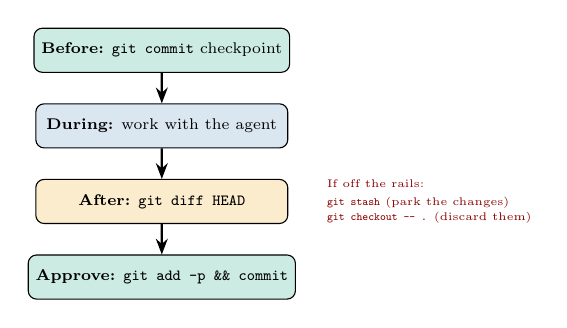
\begin{tikzpicture}[
    arr/.style={-{Stealth[length=2mm]}, thick},
    scale=0.8, transform shape
]
    \node[phase=softgreen!20] (pre) at (0,3.6)
        {\textbf{Before:} \texttt{git commit} checkpoint};
    \node[phase=softblue!20] (work) at (0,2.4)
        {\textbf{During:} work with the agent};
    \node[phase=softorange!20] (review) at (0,1.2)
        {\textbf{After:} \texttt{git diff HEAD}};
    \node[phase=softgreen!20] (commit) at (0,0)
        {\textbf{Approve:} \texttt{git add -p \&\& commit}};
    \draw[arr] (pre) -- (work);
    \draw[arr] (work) -- (review);
    \draw[arr] (review) -- (commit);
    \node[font=\tiny, text=darkred, align=left, anchor=west] at (2.5,1.2)
        {If off the rails:\\[2pt]\texttt{git stash} (park the changes)\\[1pt]\texttt{git checkout -{}- .} (discard them)};
\end{tikzpicture}
\end{center}
\begin{block}{\small Co-authors}
\scriptsize The agent is a junior contributor: its work arrives as a diff, a human reviews it before merge. Nothing it wrote is ``done'' until a person has read it.
\end{block}
\end{columns}
\end{frame}

% --- Walk-through 1: the demo project ---
\begin{frame}[fragile]{\walkthrough~1: The Demo Project in One Command~\livedemo}
\begin{columns}[T]
\column{0.50\textwidth}
\textbf{One script scaffolds the project every demo runs in:}
\begin{lstlisting}[style=bash, basicstyle=\scriptsize\ttfamily]
$ bash code/setup_demo_project.sh
# -> demo/: data, solver, CLAUDE.md,
#    deqn/, tests/, .claude/; git init
$ cd demo && claude
\end{lstlisting}
\vspace{0.4em}
\textbf{Live, the first prompt:}
\begin{lstlisting}[style=prompt, basicstyle=\scriptsize\ttfamily]
> What is in this directory? Summarise
  the structure, the two rules of CLAUDE.md
  and deqn/common.py. Write nothing yet.
\end{lstlisting}
\vspace{0.3em}
A healthy answer lists the files, names the two rules, notes the stub, and writes nothing.

\column{0.47\textwidth}
\textbf{What is in it}
\begin{lstlisting}[style=md, basicstyle=\scriptsize\ttfamily]
demo/
 CLAUDE.md             memory, two rules
 brock_mirman_reference.py  known answer
 deqn/common.py        shared, READ ONLY
 deqn/source/          the TF notebooks
 deqn/stochastic.py    stub; /goal fills it
 tests/                five tests = the exam
 reference/            reference policy; deny rule
 data/                 panel, truth, raw/
 .claude/              skills, agents,
                       settings.json
\end{lstlisting}
\end{columns}
\filebox{code/setup\_demo\_project.sh, code/CLAUDE\_md\_demo.md, code/generate\_synthetic\_data.py (the data)}
\end{frame}

\begin{frame}[fragile]{The Starting Point: A Course Notebook in TensorFlow}
\hfill\stepmarker{1}
\begin{columns}[T]
\column{0.54\textwidth}
\texttt{deqn/source/deqn\_tf\_deterministic.py}, the loss cell of the notebook ($\delta = 1$):
\begin{lstlisting}[basicstyle=\scriptsize\ttfamily]
@tf.function
def compute_cost(X, nn):
    K_t = X
    Y_t = K_t ** alpha
    s_t = nn(X)                  # savings rate
    K_tplus1 = (1. - delta) * K_t + Y_t * s_t
    C_t = Y_t - Y_t * s_t
    s_tplus1 = nn(K_tplus1)
    C_tplus1 = (1. - s_tplus1) * K_tplus1 ** alpha
    R_tplus1 = alpha * K_tplus1 ** (alpha - 1.)
    errREE = 1 - C_tplus1 / (beta * C_t * (R_tplus1 + 1. - delta))
    return tf.reduce_mean(errREE ** 2)
\end{lstlisting}

\column{0.43\textwidth}
\textbf{What it is.} The relative Euler error: zero where the household's first-order condition holds. A network for $s(K)$ is trained to make it zero on sampled $K$.

\vspace{0.5em}
\textbf{What the notebook does.} Trains for 2,000 steps and prints the loss.

\vspace{0.5em}
\textbf{What it never does.} Compare the policy with the closed form $s^* = \alpha\beta$.

\vspace{0.5em}
\begin{block}{Step 1}
Port it to PyTorch with a fixed seed, and add the check the notebook lacks.
\end{block}
\end{columns}
\filebox{code/deqn/source/ (both notebooks flattened to scripts; TensorFlow, not run here)}
\end{frame}

% ============================================================================
% PART III: THE CORE INTERACTION LOOP
% ============================================================================
\partcard{III}{The Core Interaction Loop}

% --- Feedback loop + transcript ---
\begin{frame}[fragile]{The Feedback Loop, and Where You Step In}
\hfill\stepmarker{1}
\begin{columns}[T]
\column{0.34\textwidth}
\begin{center}
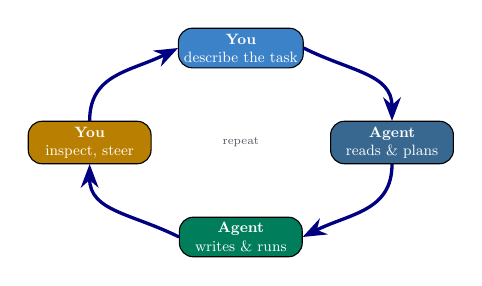
\begin{tikzpicture}[
    arr/.style={-{Stealth[length=3mm]}, very thick, uzhblue},
    scale=0.6, transform shape
]
    \node[fblock=level4] (you) at (0,2.5) {\textbf{You}\\describe the task};
    \node[fblock=softblue!80!black] (read) at (3.2,0.5) {\textbf{Agent}\\reads \& plans};
    \node[fblock=softgreen!80!black] (write) at (0,-1.5) {\textbf{Agent}\\writes \& runs};
    \node[fblock=softorange!80!black] (inspect) at (-3.2,0.5) {\textbf{You}\\inspect, steer};
    \draw[arr] (you.east) .. controls +(1,-0.5) and +(0,1) .. (read.north);
    \draw[arr] (read.south) .. controls +(0,-1) and +(1,0.5) .. (write.east);
    \draw[arr] (write.west) .. controls +(-1,0.5) and +(0,-1) .. (inspect.south);
    \draw[arr] (inspect.north) .. controls +(0,1) and +(-1,-0.5) .. (you.west);
    \node[font=\scriptsize, text=uzhgreydark] at (0,0.5) {repeat};
\end{tikzpicture}
\end{center}
\vspace{0.3em}
\boristip{5} Say \emph{what} and \emph{how you will know}; let the agent choose \emph{how}.

\column{0.64\textwidth}
Step 1 without a plan, condensed. Red \texttt{>} is what you type.
\begin{lstlisting}[style=prompt, basicstyle=\scriptsize\ttfamily]
> Port deqn/source/deqn_tf_deterministic.py
  to PyTorch. Print the loss.
\end{lstlisting}
\begin{lstlisting}[style=bash, basicstyle=\scriptsize\ttfamily]
[Reads the source; writes; runs: 3 s]
training loss (last 100 steps) 3.1e-07
Done: the loss has converged.
\end{lstlisting}
\begin{lstlisting}[style=prompt, basicstyle=\scriptsize\ttfamily]
> A small loss is not a small error. The
  answer is known: print max |s - alpha*beta|
  on [0.1, 1]; is it solved?
\end{lstlisting}
\vspace{0.2em}
\begin{alertblock}{The lesson}
``The loss converged'' is the agent's stopping point, not yours. Steer between turns with the question you would ask an RA. Here the error is $4.9\times10^{-4}$; in Part VIII the same stopping point hides a savings rate of 0.94 instead of 0.25.
\end{alertblock}
\end{columns}
\filebox{code/prompts.md, \S 2 (every prompt of the lecture, without the >, ready to paste)}
\end{frame}

% --- Prompt Quality ---
\begin{frame}[fragile]{The Prompt Quality Spectrum}
Four versions of the same request, Step 1. \emphc{Level 3 is always the goal.}

\vspace{0.3em}
\begin{center}
\scriptsize
\renewcommand{\arraystretch}{1.2}
\begin{tabular}{c p{2.4cm} p{9.4cm}}
\toprule
\textbf{Level} & \textbf{Type} & \textbf{Example} \\
\midrule
\textcolor{darkred}{\textbf{0}} & Vague & \texttt{> Port this notebook to PyTorch} \\
\textbf{1} & Specific & \texttt{> Port deqn/source/deqn\_tf\_deterministic.py to deqn/deterministic.py, same recipe: delta = 1, K \textasciitilde{} U[0.1, 1], 64 states per step, Adam 1e-3, 2000 steps.} \\
\textbf{2} & + Context & \texttt{> delta = 1, so the answer is known: s* = alpha*beta = 0.3564. The network outputs the savings rate. Use make\_net and save\_policy from deqn/common.py.} \\
\rowcolor{softgreen!10}
\textcolor{darkgreen}{\textbf{3}} & \textbf{+ Constraints, output, verification} & \texttt{> float64, seed 42. Do NOT put the closed form in the loss. Save results/deqn\_deterministic.pt with its sidecar. Verify: max |s(K) - alpha*beta| on 1,001 points < 1e-2; print it.} \\
\bottomrule
\end{tabular}
\end{center}

\vspace{0.5em}
\begin{columns}[T]
\column{0.48\textwidth}
\textbf{What makes Level 3 different}
\begin{itemize}\itemsep2pt
  \item Exact files, method, and what NOT to do
  \item Output format and location
  \item A verification step the agent runs and reports
\end{itemize}
\column{0.48\textwidth}
\boristip{6} \textbf{Challenge the agent}
\begin{itemize}\itemsep2pt
  \item ``Grill me on these changes; don't commit until I pass your test.''
  \item ``Knowing everything you know now, scrap this and implement the elegant solution.''
\end{itemize}
\end{columns}
\end{frame}

% --- Level 3 in detail + response ---
\begin{frame}[fragile]{A Level-3 Prompt and What Comes Back}
\hfill\stepmarker{1}
\begin{columns}[T]
\column{0.56\textwidth}
\textbf{The prompt}
\begin{lstlisting}[style=prompt, basicstyle=\scriptsize\ttfamily]
> Port deqn/source/deqn_tf_deterministic.py
  to deqn/deterministic.py in PyTorch, same
  recipe: delta = 1, beta = 0.99, K ~ U[0.1, 1],
  64 states per step, Adam 1e-3, 2000 steps;
  network: common.make_net(1), 1-32-32-1 tanh
  - float64; torch.manual_seed(42) first
  - loss = mean squared relative Euler error;
    do NOT put the closed form in it
  - save results/deqn_deterministic.pt
  Verify: max |s(K) - alpha*beta| on 1,001
  points of [0.1, 1] < 1e-2; print it.
\end{lstlisting}

\column{0.41\textwidth}
\textbf{The response} (condensed; the numbers are the committed script's)
\begin{lstlisting}[style=bash, basicstyle=\scriptsize\ttfamily]
[Read the source, common.py]
[Wrote deqn/deterministic.py]
[Ran it: 3.2 s]
loss (last 100) 3.1e-07
max |s - alpha*beta|: 4.91e-04
assert < 1e-2: OK
[Wrote results/...pt]
\end{lstlisting}
\vspace{0.3em}
\begin{block}{Why this is Level 3}
No re-prompt for the check, the file or the seed: each was specified up front and delivered in one pass. The answer arrived with its own grade.
\end{block}
\end{columns}
\textbf{The residual it wrote} is the TensorFlow cell of the previous slide, line for line, in PyTorch.
\filebox{code/deqn/deterministic.py; the prompt: code/prompts.md, \S 3}
\end{frame}

% --- Live demo: plan mode ---
\begin{frame}[fragile]{Step 1 in Plan Mode~\livedemo}
\footnotesize
\stepmarker{1}\par\vspace{0.1em}
\textbf{Shift+Tab} until the prompt shows \texttt{[plan]}: the agent reads, but writes nothing until the plan is approved.
\begin{lstlisting}[style=prompt, basicstyle=\scriptsize\ttfamily]
> Step 1 of the DEQN build. deqn/source/deqn_tf_deterministic.py is a course
  notebook: a network for the savings rate, delta = 1, trained on the Euler
  residual. The answer is known: s* = alpha*beta. Say how you would port it:
  1. deqn/deterministic.py: PyTorch, float64, seed 42, same recipe, make_net(1)
  2. scripts/check_step1.py: max |s(K) - alpha*beta| and the residual, 1,001 pts
  3. figures/deqn_step1.pdf: s(K) vs alpha*beta; |residual| on a log axis
  4. notes/deqn_step1.md: three sentences: is it solved, and how can you tell
  Do NOT use the closed form outside the check. Do NOT modify deqn/common.py.
\end{lstlisting}
\vspace{0.2em}
\begin{columns}[T]
\column{0.52\textwidth}
\textbf{Read the plan before approving it}
\begin{itemize}\itemsep2pt
  \item Every file it will create, and nothing else?
  \item The closed form only in the check, not in the loss?
  \item ``Solved'' judged by the max error, or by the loss?
\end{itemize}
\textbf{A good run:} four files in one pass; max error $4.9\times10^{-4}$ against a threshold of $10^{-2}$.
\column{0.45\textwidth}
\begin{center}
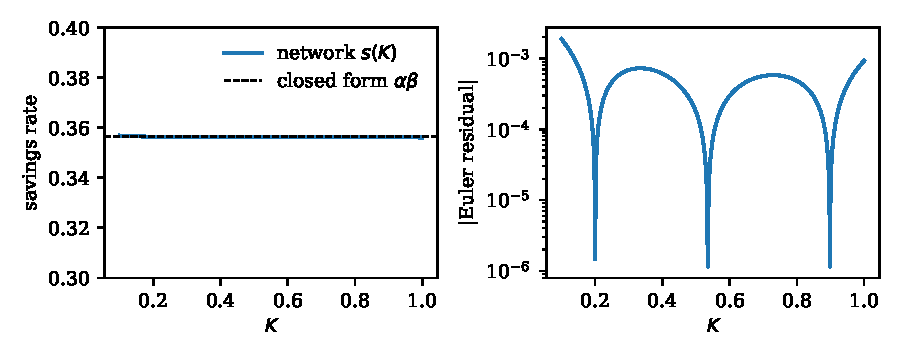
\includegraphics[width=0.9\linewidth]{figures/agentic_deqn_step1.pdf}
\end{center}
\end{columns}
\filebox{code/prompts.md, \S 4 (the prompt and the expected numbers); our version: code/deqn/deterministic.py}
\end{frame}

% --- Agents and notebooks ---
\begin{frame}[fragile]{Agents and Jupyter Notebooks}
Much of economics lives in notebooks. The agent reads, edits and runs them; three habits are worth fixing from the start.

\vspace{0.4em}
\begin{columns}[T]
\column{0.50\textwidth}
\textbf{What the agent does with an \texttt{.ipynb}}
\begin{itemize}\itemsep3pt
  \item Reads it cell by cell, \emph{outputs included}: a stored result is evidence it can quote
  \item Edits one cell at a time; a hook can log or block that like any file edit
  \item Runs it headless (no interface, as a batch job) when asked:
\end{itemize}
\begin{lstlisting}[style=bash, basicstyle=\scriptsize\ttfamily]
jupyter nbconvert --to notebook --execute \
   --output out.ipynb estimation.ipynb
\end{lstlisting}

\column{0.47\textwidth}
\textbf{Three habits}
\begin{enumerate}\itemsep3pt
  \item \emphc{One notebook per session}; \texttt{/clear} between them. Outputs and figures are a large context load.
  \item \emphc{Set the budget before you run}: keep the smoke-test settings; expose sample sizes in the first cell.
  \item \emphc{Verify against the stored result}: a table ``stored vs fresh'' and a verdict, never ``it works''.
\end{enumerate}
\end{columns}

\vspace{0.5em}
\begin{block}{Better still}
Port the notebook into a script with tests, as Step 1 did. The notebook stays for exploration; the paper runs from the script.
\end{block}
\filebox{code/prompts.md, \S 5 (the headless-run prompt)}
\end{frame}

% --- Parallel sessions ---
\begin{frame}[fragile]{Parallel Sessions and Git Worktrees}
\boristip{1} \textbf{Do more in parallel}, says the Claude Code team. The evidence is mixed (Brynjolfsson et al., 2025: gains for novices; METR, 2025: experts slower): time yourself.

\vspace{0.4em}
\begin{columns}[T]
\column{0.50\textwidth}
A \emphc{worktree} is a second checkout of the same repository in a sibling folder, on its own branch. Each gets its own session, each session its own files:
\begin{lstlisting}[style=bash, basicstyle=\scriptsize\ttfamily]
git worktree add ../a -b data-clean
git worktree add ../b -b estimation
git worktree add ../c -b lit-review
cd ../a && claude    # terminal 1
cd ../b && claude    # terminal 2
\end{lstlisting}
\vspace{0.3em}
Say the scope in each session: ``only modify files under \texttt{code/}''. Merging is cheap because the files do not overlap.

\column{0.46\textwidth}
\begin{center}
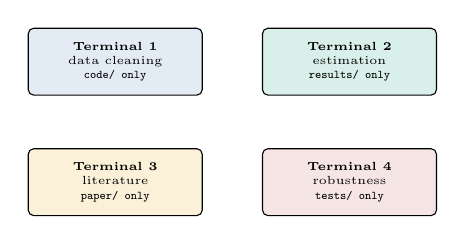
\begin{tikzpicture}[scale=0.85, transform shape]
    \node[tpane=softblue!15] (t1) at (0,0)
        {\textbf{Terminal 1}\\data cleaning\\{\ttfamily code/ only}};
    \node[tpane=softgreen!15] (t2) at (3.5,0)
        {\textbf{Terminal 2}\\estimation\\{\ttfamily results/ only}};
    \node[tpane=softorange!15] (t3) at (0,-1.8)
        {\textbf{Terminal 3}\\literature\\{\ttfamily paper/ only}};
    \node[tpane=harvardcrimson!10] (t4) at (3.5,-1.8)
        {\textbf{Terminal 4}\\robustness\\{\ttfamily tests/ only}};
\end{tikzpicture}
\end{center}
\vspace{0.3em}
\textcolor{darkred}{\textbf{Cost:}} parallel sessions consume quota in parallel; Max or pay-as-you-go API is the realistic tier for this.
\end{columns}
\end{frame}

% --- Context management in practice ---
\begin{frame}[fragile]{Context Management in Practice}
\begin{columns}[T]
\column{0.48\textwidth}
\textbf{The progress-file pattern}, for any session beyond ten turns:
\begin{lstlisting}[style=prompt, basicstyle=\scriptsize\ttfamily]
> Write notes/session_state.md:
  1. What we have done so far
  2. What is working
  3. What we need to do next
  4. Design decisions and why
\end{lstlisting}
Next session:
\begin{lstlisting}[style=prompt, basicstyle=\scriptsize\ttfamily]
> Read notes/session_state.md and
  continue from where we left off.
\end{lstlisting}

\vspace{0.3em}
\textbf{Resuming sessions:}
\begin{itemize}\itemsep0pt
    \item \texttt{claude -{}-continue}: resume the last session
    \item \texttt{claude -{}-resume}: pick from recent sessions
    \item \texttt{/rename "estimation pipeline"}: name a session for later
\end{itemize}

\column{0.48\textwidth}
\textbf{When to use which approach:}

\vspace{0.2em}
\scriptsize
\renewcommand{\arraystretch}{1.2}
\begin{tabular}{p{1.9cm} p{3.9cm}}
\toprule
\textbf{Situation} & \textbf{Action} \\
\midrule
$<5$ turns & just work \\
5--15 turns & write the progress file at the end \\
\texttt{/context} at 60\,\% & \texttt{/compact} + progress file \\
New sub-task & \texttt{/clear} or a new session \\
Reading-heavy research & delegate to a \emphc{subagent}; only its summary enters your window \\
\bottomrule
\end{tabular}

\normalsize
\vspace{0.4em}
\begin{block}{\small The principle}
\scriptsize Memory between sessions lives on disk and in git, never in the conversation. Everything you would want a new RA to know on Monday morning goes into a file.
\end{block}
\end{columns}
\filebox{code/prompts.md, \S 6}
\end{frame}

% ============================================================================
% PART IV: PROMPT ENGINEERING FOR RESEARCH
% ============================================================================
\partcard{IV}{Prompt Engineering for Research}

% --- Anatomy + before/after ---
\begin{frame}[fragile]{Anatomy of a Research Prompt: Six Components}
\begin{center}
\small
\renewcommand{\arraystretch}{1.2}
\begin{tabular}{c l p{4.6cm} p{4.6cm}}
\toprule
\textbf{\#} & \textbf{Component} & \textbf{What it does} & \textbf{Failure if missing} \\
\midrule
1 & \textbf{Role} & who the agent is here & generic output \\
2 & \textbf{Context} & what it needs to know & asks too many questions \\
3 & \textbf{Task} & what you want done & invents another task \\
4 & \textbf{Constraints} & must / must not & ``AI's code'', not yours \\
5 & \textbf{Output} & deliverable, format, location & wrong format, extra junk \\
6 & \textbf{Verification} & how to check it & plausible but wrong \\
\bottomrule
\end{tabular}
\end{center}

\vspace{0.5em}
\begin{columns}[T]
\column{0.48\textwidth}
\textbf{Before} (Level 0, everything missing):
\begin{lstlisting}[style=prompt, basicstyle=\small\ttfamily]
> Add productivity shocks to the solver.
\end{lstlisting}
\column{0.48\textwidth}
\begin{block}{The meta-rule}
When something goes wrong, ask ``which of the six did I omit?'' The answer is almost always the fix.
\end{block}
\end{columns}
\vspace{0.3em}
\textbf{After:} next slide, the same task with all six, which is Step 2 of the lead example. Level 3 of the prompt spectrum is all six components present.
\end{frame}

\begin{frame}[fragile]{The Six Components, Filled In: Step 2, the Stochastic Solver}
\footnotesize
\hfill\stepmarker{2}
\begin{lstlisting}[style=md, basicstyle=\scriptsize\ttfamily]
[ROLE]        You are a computational macroeconomist.
[CONTEXT]     deqn/deterministic.py (Step 1) is verified against the closed form. Now the
              stochastic model of CLAUDE.md; no closed form; the reference is
              brock_mirman_reference.solve(0.96, 0.9). Read the docstring of deqn/common.py first.
[TASK]        Write deqn/stochastic.py with solve(seed=42, steps=2000): state (log z / sd_z,
              log K - log K*); network 2-32-32-1 tanh, sigmoid output, s_init = s*; loss = mean
              squared Euler residual with the 5 Gauss-Hermite nodes; 128 fresh states per step.
[CONSTRAINTS] torch, float64, torch.manual_seed(seed) first. Never use the reference policy in
              a loss or an initialisation. Do not modify deqn/common.py, tests/ or reference/.
[OUTPUT]      results/deqn_stochastic.pt with its JSON sidecar; solve returns {"s", "net", "wall"}.
[VERIFY]      Simulate 2,000 periods with the network's own policy. Report mean |residual| there,
              max |s - s_ref| at those states, E[s] against the reference, and whether log K stayed inside
              [log K* - 0.5, log K* + 0.5]. Then run python3 -m pytest -q tests/ and show it.
\end{lstlisting}
\vspace{0.3em}
\begin{columns}[T]
\column{0.48\textwidth}
\textbf{Verification is the longest part}, and the only part the agent cannot invent: the path its own policy generates, the reference, the window.
\column{0.48\textwidth}
\textbf{Not run now.} The same text returns as the recipe of the \texttt{/goal} in Part VII (Step 4) and as the plan of Part VIII (Step 5): one solver, built three ways.
\end{columns}
\filebox{code/prompts.md, \S 7 (this prompt, copy-paste ready, and the six templates)}
\end{frame}

% --- Constraints ---
\begin{frame}[fragile]{The Constraint Vocabulary}
\footnotesize
Constraints are the difference between ``AI wrote the code'' and ``AI wrote \emphc{my} code''. The constraint lines of Step 2:

\vspace{0.4em}
\begin{columns}[T]
\column{0.32\textwidth}
\textbf{\textcolor{darkred}{Negative}}: what NOT to do
\begin{lstlisting}[style=prompt, basicstyle=\scriptsize\ttfamily]
Do NOT use reference/ in
  a loss, an init or a fit.
Do NOT edit tests/ or
  reference/.
Do NOT report the training
  loss as accuracy.
\end{lstlisting}
\column{0.32\textwidth}
\textbf{\textcolor{darkgreen}{Positive}}: what to do
\begin{lstlisting}[style=prompt, basicstyle=\scriptsize\ttfamily]
Use deqn/common.py: make_net,
  encode_state, save_policy.
float64; seed torch before
  the network.
Notation of CLAUDE.md:
  K, z, s, rho, K*, s*.
\end{lstlisting}
\column{0.32\textwidth}
\textbf{\textcolor{uzhblue}{Scope}}: boundaries
\begin{lstlisting}[style=prompt, basicstyle=\scriptsize\ttfamily]
Only write deqn/stochastic.py
  and results/.
Make the minimum change that
  fixes the failing test.
Stop and report after each
  pytest run.
\end{lstlisting}
\end{columns}

\vspace{0.6em}
\begin{alertblock}{The ``think before you code'' pattern}
``BEFORE writing any code: (1) describe your plan, (2) list every file you will modify, (3) list the risks. Do not proceed until I say `go ahead'.'' Plan mode does this for you; the sentence does it in any tool.
\end{alertblock}
\filebox{code/prompts.md, \S 7 (the constraint lines, ready to append to any prompt)}
\end{frame}

% --- Templates I ---
\begin{frame}[fragile]{Prompt Templates I: Replication, Robustness, Autonomy, Writing}
\footnotesize
Four prompts you will type more than once. The full text of each is in the repository.

\vspace{0.4em}
\begin{columns}[T]
\column{0.48\textwidth}
\begin{block}{1. Replication check, code vs paper}
``Read \texttt{code/estimate.py} and Section 3 of the paper. Does the estimator in the code match the paper? One line per item: \checkmark{} matches, $\times$ paper says X / code does Y, ? unclear.''
\end{block}
\begin{block}{3. Autonomous session}
``I am away for 30 minutes. Implement the pipeline per \texttt{plan.md}. Commit after each step. If stuck after 3 attempts, write \texttt{notes/blocked.md} and STOP. Do NOT touch the raw data.''
\end{block}
\column{0.48\textwidth}
\begin{block}{2. Robustness table}
``Add three checks to the baseline: drop post-2008, cluster by region, region trends. One script each, results to \texttt{results/robustness\_\{name\}.json}, then one booktabs table with all four columns.''
\end{block}
\begin{block}{4. Literature writing}
``Do NOT invent citations. Cite only \texttt{paper/references.bib}. If a claim needs a source that is not there, write \texttt{[CITE: author, year -{}- verify]} and list the gaps at the end.''
\end{block}
\end{columns}
\vspace{0.3em}
Every one of them names the files, the output and the stopping rule. That is what makes them reusable.
\filebox{code/prompts.md, \S 7, templates 1--4 (verbatim, copy-paste ready)}
\end{frame}

% --- Templates II ---
\begin{frame}[fragile]{Prompt Templates II: Turn ``Is This Right?'' into a Number}
\footnotesize
\begin{columns}[T]
\column{0.49\textwidth}
\begin{block}{5. Translate legacy code, and prove it}
``Port \texttt{deqn/source/deqn\_tf\_stochastic.py} (TensorFlow) to PyTorch. Do NOT change the algorithm. Then write tests: the residual has shape $(n, 1)$; the quadrature weights sum to 1; at $\sigma = 0$ and $\delta = 1$ it reduces to the Euler equation of Step 1. Report every deviation with the line that causes it.''
\end{block}
The original has \texttt{expectation = tf.zeros((n\_data, dim\_state))}: two identical residual columns, the loss unchanged, never noticed in training. The first test catches it. The notebook's $\beta = 0.99$ becomes the 0.96 of \texttt{CLAUDE.md}.
\column{0.49\textwidth}
\begin{block}{6. Check a derivation with computer algebra}
``Derive the Euler equation and the steady state $(K^*, s^*)$ of the model in \texttt{CLAUDE.md}. Verify every step with sympy in \texttt{notes/check\_euler.py}: substitute the steady state into the Euler equation and print the residual, which must be 0. Cross-check $K^*$ against \texttt{steady\_state(0.96)}. If a residual is not zero, say so; do not adjust the derivation to fit.''
\end{block}
Reference: $K^* = 4.294$, $s^* = 0.254$. That Euler equation is the DEQN's residual.
\end{columns}

\vspace{0.5em}
\begin{alertblock}{The pattern}
Both templates turn ``is this right?'' into a number that is zero when it is. That is what makes an agent safe to use on a model.
\end{alertblock}
\filebox{code/prompts.md, \S 7, templates 5--6}
\end{frame}

% --- Failure modes ---
\begin{frame}{Common Failure Modes and Their Fixes}
\begin{center}
\small
\renewcommand{\arraystretch}{1.15}
\begin{tabular}{p{4.0cm} p{3.2cm} p{5.4cm}}
\toprule
\textbf{Failure} & \textbf{Cause} & \textbf{Fix} \\
\midrule
The agent ``invents'' results & vague output spec & an explicit verification step \\
Modifies the wrong files & no scope constraint & an explicit file scope \\
Long session degrades & context overflow & \texttt{/compact}; break into sessions \\
Loops on the same error & no retry limit & ``if 3 attempts fail, stop and write blocked.md'' \\
Wrong solution method & no domain context & name the method, point to the paper section \\
Loss converges, solution wrong & the only check was the loss & on-path residuals and the reference policy (Part VIII) \\
Over-specified \texttt{CLAUDE.md} & too many instructions & under 200 lines; rules into hooks \\
\bottomrule
\end{tabular}
\end{center}

\vspace{0.6em}
\begin{alertblock}{The highest-leverage fix}
\emphc{Give the agent a way to verify its own work}: tests, expected outputs, or synthetic data with a known answer. It prevents most failures, and it is the theme of Block 2.
\end{alertblock}
\end{frame}

% ============================================================================
% BREAK
% ============================================================================
\begin{frame}{}
\vfill
\begin{center}
{\Huge \textcolor{uzhblue}{\textbf{Break}}}\\[12pt]
{\LARGE 10 minutes}\\[16pt]
{\small Block 2: extending the agent with \texttt{CLAUDE.md}, skills, subagents and hooks; closing the loop with \texttt{/goal};\\from plan to table and figure; verification, disclosure and governance.}
\end{center}
\vfill
\end{frame}

% ============================================================================
% PART V: PROJECT MEMORY & CLAUDE.md
% ============================================================================
\partcard{V}{Project Memory: \texttt{CLAUDE.md}}

% --- What is CLAUDE.md ---
\begin{frame}{What Is \texttt{CLAUDE.md}?}
\footnotesize
\texttt{CLAUDE.md} is read \emphc{automatically} at session start: your project's persistent memory for a capable but amnesiac research assistant.

\vspace{0.4em}
\begin{columns}[T]
\column{0.50\textwidth}
\textbf{Where it lives}
\begin{itemize}\itemsep2pt
  \item \texttt{\textasciitilde/.claude/CLAUDE.md}: you, across all projects
  \item \texttt{./CLAUDE.md}: the project, in git, shared with co-authors
  \item \texttt{.claude/rules/*.md}: rules scoped to paths
\end{itemize}
\vspace{0.3em}
\textbf{Highest-value sections}
\begin{enumerate}\itemsep2pt
  \item Repository structure, with the read-only directories
  \item Coding standards and statistical conventions
  \item Notation, matching the paper
  \item Current status, updated every session
  \item A ``do not touch'' list
\end{enumerate}
\column{0.46\textwidth}
\boristip{3} \textbf{Invest in your \texttt{CLAUDE.md}.} After every correction:
\begin{center}
\fcolorbox{harvardcrimson}{red!5}{%
\parbox{5.4cm}{\centering\itshape
``Update CLAUDE.md so you don't\\make that mistake again.''}}
\end{center}
\vspace{0.3em}
\textbf{Three rules} (Claude Code docs)
\begin{itemize}\itemsep2pt
  \item Under 200 lines: it is in the context of every turn
  \item Preferences in \texttt{CLAUDE.md}; \emphc{critical} rules in hooks (Part VI): a text file is a request, not a guarantee
  \item Write it for a new RA on Monday morning
\end{itemize}
\end{columns}
\vspace{0.3em}
{\scriptsize\textcolor{uzhgreydark}{\texttt{/init} writes a first draft from your repository; \texttt{/memory} shows it together with the agent's own auto-memory.}}
\end{frame}

% --- Walk-through 2: CLAUDE_md_template ---
\begin{frame}[fragile]{\walkthrough~2: A Filled-in \texttt{CLAUDE.md}}
\footnotesize
Left: a fictional paper under revision. Right: the demo project's own file, the part that governs the solver.
\begin{columns}[T]
\column{0.49\textwidth}
\begin{lstlisting}[style=md, basicstyle=\scriptsize\ttfamily]
# CLAUDE.md -- Fiscal Multipliers in a HANK Model
## Project Overview
- Stage: Revision (R&R at Review of Economic Studies)
## Repository Structure
data/raw/     <- READ ONLY. Never modify.
code/estimate.py  <- SMM + neural surrogate
paper/tables/ <- generated; do not hand-edit
## Statistical Conventions
- SE clustered at the state level (51 clusters)
- Block bootstrap, block length 8 quarters, 1000 reps
## Decisions Made
- 2026-01: switched the solver to JAX
\end{lstlisting}
\column{0.49\textwidth}
\begin{lstlisting}[style=md, basicstyle=\scriptsize\ttfamily]
## The two rules of this project
1. data/bm_panel_truth.csv holds the hidden rho.
   Do not open it unless the prompt says the
   verification step has been reached.
2. reference/ and tests/ are the exam. Never load
   the reference into a loss or an initialisation;
   never edit either (a hook refuses).
## DEQN notation and standards
- s_theta(x), x = (log z / sd_z, log K - log K*)
- r = beta C E[(1 - delta + R') / C'] - 1
- Accuracy = the residual on the network's OWN
  path and the distance to the reference. The
  training loss is never reported as accuracy.
\end{lstlisting}
\end{columns}
\vspace{0.2em}
\begin{alertblock}{Spot the stale line, in the paper's file}
Its decision log says JAX; its package list (not shown) still says TensorFlow. The agent believes whichever it reads last. Update the file every session.
\end{alertblock}
\filebox{code/CLAUDE\_md\_template.md (83 lines), code/CLAUDE\_md\_demo.md (= demo/CLAUDE.md); prompt: code/prompts.md, \S 8}
\end{frame}

% ============================================================================
% PART VI: SKILLS, SUBAGENTS, HOOKS, MCP
% ============================================================================
\partcard{VI}{Skills, Subagents, Hooks, MCP}

% --- The map ---
\begin{frame}{Four Extension Mechanisms}
\footnotesize
\begin{center}
\renewcommand{\arraystretch}{1.3}
\begin{tabular}{l p{3.8cm} p{3.9cm} p{3.0cm}}
\toprule
\textbf{Mechanism} & \textbf{What it is} & \textbf{Lives at} & \textbf{Use when} \\
\midrule
\emphc{Skill} & a workflow in a Markdown file; a slash command & \texttt{.claude/skills/\allowbreak<name>/\allowbreak SKILL.md} & you type the same sequence twice a day \\
\emphc{Subagent} & a specialist with its own prompt, tools, model and context window & \texttt{.claude/agents/\allowbreak<name>.md} & fresh context or an independent reviewer \\
\emphc{Hook} & a shell command fired on events (\texttt{PreToolUse}, \texttt{PostToolUse}, \dots) & \texttt{.claude/settings.json} & deterministic enforcement: block a path, run a linter, log \\
\emphc{MCP server} & an external service exposing tools & out of process; \texttt{claude mcp add} & data or actions outside the project \\
\bottomrule
\end{tabular}
\end{center}

\vspace{0.6em}
\textbf{Rule of thumb.} Skills package prompts; subagents package specialists; hooks enforce policy; MCP plugs in external worlds. All four are plain files in your repository, versioned and shared like code. \texttt{/goal} (Part VII) wraps them into a closed loop.
\end{frame}

% --- Walk-through 3: skills ---
\begin{frame}[fragile]{\walkthrough~3: Skills~\livedemo}
\footnotesize
\hfill\stepmarker{3}
\boristip{4} \textbf{If you do something more than once a day, turn it into a skill}: a Markdown file of instructions, invoked by name, with scripts next to it.
\begin{columns}[T]
\column{0.52\textwidth}
\texttt{/deqn-accuracy}, the on-path check of a saved policy:
\begin{lstlisting}[style=md, basicstyle=\scriptsize\ttfamily]
---
name: deqn-accuracy
description: Audit a saved DEQN policy on the
  path its own policy generates: residuals,
  distance to the reference, E[s], the window.
---
### Step 1  Identify the .pt file
### Step 2  Run the check
  python3 .claude/skills/deqn-accuracy/\
          accuracy.py <pt>
### Step 3  Report the lines verbatim, then
  one sentence and the verdict
### Step 4  Save notes/accuracy_<file>.{md,pdf}
## Constraints
- Never retrain; never quote the training
  loss as accuracy.
\end{lstlisting}
\column{0.45\textwidth}
\textbf{Live:} \texttt{/deqn-accuracy results/deqn\_deterministic.pt}
\begin{lstlisting}[style=bash, basicstyle=\scriptsize\ttfamily]
reference: closed form s* = 0.3564
|Euler residual| on the grid:
   mean 4.68e-04  max 1.87e-03
|s - s_ref|: max 4.91e-04
E[s] = 0.3564 vs reference 0.3564
path [0.20, 0.28] in [0.10, 1.00]
verdict: ACCURATE
\end{lstlisting}
\vspace{0.3em}
The \texttt{description} is what the agent reads to decide when to invoke a skill on its own. The script next to \texttt{SKILL.md} is the same \texttt{accuracy.py} the tests and the slides use: one check, written once.

\vspace{0.2em}
Two more in the demo: \texttt{/data-diagnostics}, \texttt{/strategic-revision}.
\end{columns}
\filebox{code/skills/deqn-accuracy/SKILL.md, code/deqn/accuracy.py (109 lines); prompts: code/prompts.md, \S 9}
\end{frame}

% --- Walk-through 4: subagents ---
\begin{frame}[fragile]{\walkthrough~4: Subagents~\livedemo}
\footnotesize
\boristip{8} \textbf{Use subagents} to throw more compute at a problem and keep your main context clean.
\begin{columns}[T]
\column{0.50\textwidth}
\texttt{.claude/agents/verifier.md}, abridged:
\begin{lstlisting}[style=md, basicstyle=\scriptsize\ttfamily]
---
name: verifier
description: Read-only skeptic: is a claimed
  result supported by files and outputs?
model: haiku
tools: Read, Grep, Glob
---
# Verifier
1. Restate the claim in one sentence.
2. Inspect only the files and outputs needed.
3. Report each claim as PASS, FAIL or UNSURE.
4. End with the smallest follow-up checks.
## Constraints
- Never modify files. Never declare success
  without pointing to concrete evidence.
\end{lstlisting}
\textbf{Live:} \texttt{> Use the verifier subagent to check the claims in the accuracy report under notes/.}
\column{0.46\textwidth}
\textbf{The frontmatter}
\begin{itemize}\itemsep2pt
  \item \texttt{description}: when the main agent delegates
  \item \texttt{model}: pay for what the role needs (\texttt{haiku} here)
  \item \texttt{tools}: a whitelist; read-only means no \texttt{Bash}, \texttt{Edit}, \texttt{Write}
  \item its own context window; only a summary comes back
\end{itemize}
\vspace{0.4em}
\begin{block}{Golden rule}
One responsibility per subagent. The main session builds; a \emph{different} agent with a \emph{different} prompt checks. That is what makes the verifier worth having.
\end{block}
\vspace{0.3em}
The demo ships eight (list on the quick-reference card).
\end{columns}
\filebox{code/agents/*.md (8 files), installed to demo/.claude/agents/; prompts: code/prompts.md, \S 9}
\end{frame}

% --- Specialists ---
\begin{frame}[fragile]{Specialists, Not Generic Reviewers}
\footnotesize
A generic reviewer checks that code runs. A specialist knows what \emph{runs cleanly and is still wrong}.
\begin{columns}[T]
\column{0.50\textwidth}
\texttt{solution-accuracy-checker}: is a solved model actually solved?
\begin{lstlisting}[style=md, basicstyle=\scriptsize\ttfamily]
## Four checks, in this order
1. Residuals on a held-out test set: states
   the solver did NOT train on.
2. Against a reference: compare the POLICY.
   A small residual with a large policy
   error is the finding (silent_failure.md).
3. Extrapolation: the policy 2 sd outside
   the ergodic set; still economic sense?
4. Reproducibility: seed, versions, wall-
   clock recorded next to the result?
Verdict: ACCURATE / DEGRADED / WRONG
\end{lstlisting}
\begin{lstlisting}[style=prompt, basicstyle=\scriptsize\ttfamily]
> Use solution-accuracy-checker on
  results/deqn_stochastic.pt.
\end{lstlisting}
\column{0.46\textwidth}
\texttt{econometrics-reviewer}: the applied economist's checklist
\begin{lstlisting}[style=md, basicstyle=\scriptsize\ttfamily]
### A. Identification
- The identifying assumption, one sentence.
- DiD: pre-trends? heterogeneous effects
  (Callaway-Sant'Anna, Sun-Abraham)?
- IV: effective first-stage F (Montiel
  Olea-Pflueger); F < 10 not sufficient.
- RDD: bandwidth, polynomial, manipulation.
### B. Controls  C. Clustering  D. Sample
Verdict: APPROVE / REQUEST CHANGES / BLOCK
\end{lstlisting}
\vspace{0.2em}
\begin{alertblock}{Why specialists}
A converged loss next to a wrong policy, a weak first stage behind a significant coefficient: both \emph{run cleanly}.
\end{alertblock}
\end{columns}
\filebox{code/agents/solution\_accuracy\_checker.md, econometrics\_reviewer.md, loss\_balancing\_reviewer.md; prompts: code/prompts.md, \S 9}
\end{frame}

% --- Walk-through 5: deny rules and hooks ---
\begin{frame}[fragile]{\walkthrough~5: Deny Rules and Hooks}
\footnotesize
\begin{columns}[T]
\column{0.42\textwidth}
Two mechanisms in one settings file, for two problems.

\vspace{0.4em}
\textbf{Deny rules} decide what the agent may \emph{read}. A denied file is never opened, so its content never reaches the API: the confidentiality tool. Here: \texttt{data/raw/} and the reference policy.

\vspace{0.4em}
\textbf{Hooks} are shell commands around the agent's tool calls. A \texttt{PreToolUse} hook that exits 2 \emph{blocks} the call. Here: no edits under \texttt{data/raw/}, \texttt{reference/}, \texttt{tests/}: the exam the \texttt{/goal} works against.

\vspace{0.4em}
\begin{alertblock}{The point}
\texttt{CLAUDE.md} asks; the rule enforces. Preferences in text, rules in code.
\end{alertblock}
\column{0.56\textwidth}
\begin{lstlisting}[style=json, basicstyle=\scriptsize\ttfamily]
"permissions": { "deny": [
    "Read(./data/raw/**)",  "Bash(cat data/raw/*)",
    "Read(./reference/**)", "Bash(cat reference/*)" ] },
"hooks": { "PreToolUse": [{
    "matcher": "Edit|Write|MultiEdit|NotebookEdit",
    "hooks": [{ "type": "command",
      "command": "jq -e '.tool_input.file_path
         | test(\"(^|/)(data/raw|reference|tests)/\")'
         > /dev/null && { echo 'read-only per
         CLAUDE.md' >&2; exit 2; }; exit 0" }] }],
  "PostToolUse": [{  /* ruff, latexmk, audit log */ }] }
\end{lstlisting}
\textbf{Live (optional):} \texttt{> Relax the threshold in tests/test\_deqn\_stochastic.py to 0.1} (the hook refuses); \texttt{> Show me reference/baseline.md} (the deny rule refuses).
\end{columns}
\filebox{code/hooks/settings.json (64 lines, needs jq) = demo/.claude/settings.json; docs: code.claude.com/docs/en/hooks-guide}
\end{frame}

% --- MCP ---
\begin{frame}[fragile]{MCP: Connecting the Agent to External Tools}
\footnotesize
The \textbf{Model Context Protocol} connects the agent to services outside the project tree: Tier 3 becomes Tier 4.

\vspace{0.3em}
\begin{columns}[T]
\column{0.50\textwidth}
\begin{lstlisting}[style=bash, basicstyle=\scriptsize\ttfamily]
# a remote server (token header: see docs)
claude mcp add --transport http github \
    https://api.githubcopilot.com/mcp/
# a local server: any command speaking MCP
claude mcp add --transport stdio zotero \
    -- npx -y <package>
claude mcp list     # /mcp inside a session
\end{lstlisting}
\vspace{0.3em}
\begin{lstlisting}[style=prompt, basicstyle=\scriptsize\ttfamily]
> Search Zotero for papers on fiscal multipliers
  in HANK models; list the ones not yet in
  paper/references.bib
\end{lstlisting}
\vspace{0.3em}
\boristip{9} With a database CLI or MCP server, the agent pulls and analyses the data. Boris Cherny: ``I haven't written SQL in six months.''
\column{0.46\textwidth}
\begin{center}
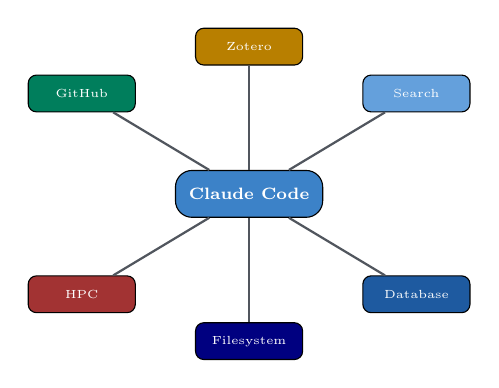
\begin{tikzpicture}[conn/.style={thick, uzhgreydark}, scale=0.85, transform shape]
    \node[draw, rounded corners=6pt, fill=level4,
          minimum width=2.2cm, minimum height=0.7cm,
          font=\scriptsize\bfseries, text=white] (cc) at (0,0) {Claude Code};
    \node[spoke=softgreen!80!black] (git) at (-2.5,1.5) {GitHub};
    \node[spoke=softorange!80!black] (zot) at (0,2.2) {Zotero};
    \node[spoke=level3] (search) at (2.5,1.5) {Search};
    \node[spoke=darkred!80] (hpc) at (-2.5,-1.5) {HPC};
    \node[spoke=uzhblue] (fs) at (0,-2.2) {Filesystem};
    \node[spoke=level5] (db) at (2.5,-1.5) {Database};
    \foreach \s in {git,zot,search,hpc,fs,db} \draw[conn] (cc) -- (\s);
\end{tikzpicture}
\end{center}
Whatever a tool \emph{returns} enters the context, and therefore the API call. For an institute, the interesting servers are its data and compute platforms (Part IX).
\end{columns}
\filebox{code/prompts.md, \S 10}
\end{frame}

% ============================================================================
% PART VII: AUTONOMOUS LOOPS
% ============================================================================
\partcard{VII}{Autonomous Loops}

% --- Closing the loop: the pattern and three mechanisms ---
\begin{frame}{Closing the Loop: The Pattern, and Three Ways to Run It}
\footnotesize
So far a human was in the loop. The next move is to \emphc{close it}: a verifier, not a person, decides when the task is done.
\vspace{0.1em}
\begin{center}
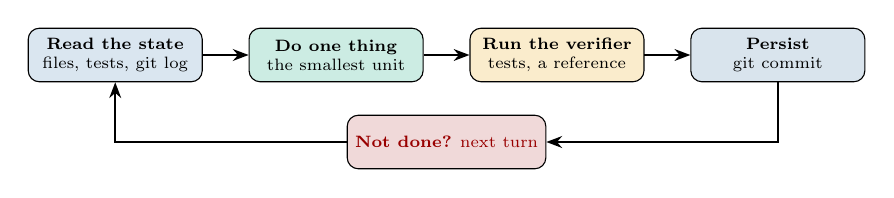
\begin{tikzpicture}[
    box/.style={draw, rounded corners=4pt, minimum width=2.6cm, minimum height=0.8cm, font=\scriptsize, align=center},
    arr/.style={-{Stealth[length=2mm]}, thick}, scale=0.85, transform shape]
    \node[box, fill=softblue!20]   (wake)  at (0,0)    {\textbf{Read the state}\\files, tests, git log};
    \node[box, fill=softgreen!20]  (work)  at (3.3,0)  {\textbf{Do one thing}\\the smallest unit};
    \node[box, fill=softorange!20] (check) at (6.6,0)  {\textbf{Run the verifier}\\tests, a reference};
    \node[box, fill=level1!50]     (commit)at (9.9,0)  {\textbf{Persist}\\git commit};
    \node[box, fill=harvardcrimson!15, text=harvardcrimson] (next) at (4.95,-1.3) {\textbf{Not done?} next turn};
    \draw[arr] (wake) -- (work); \draw[arr] (work) -- (check); \draw[arr] (check) -- (commit);
    \draw[arr] (commit) |- (next); \draw[arr] (next) -| (wake);
\end{tikzpicture}
\end{center}

\vspace{0.3em}
\begin{center}
\renewcommand{\arraystretch}{1.25}
\begin{tabular}{@{}p{3.4cm} p{2.9cm} p{2.9cm} p{3.4cm}@{}}
\toprule
\textbf{Mechanism} & \textbf{Next turn starts when} & \textbf{Context} & \textbf{Stops when} \\
\midrule
\emphc{\texttt{/goal <condition>}} (today) & the previous turn ends & same session & a separate evaluator judges the condition met \\
\texttt{/loop [interval] <prompt>} & a timer fires & same session & you stop it, or the agent decides \\
a shell loop over \texttt{claude -p} (the ``Ralph loop'') & your script calls it again & a fresh process; disk is the memory & your test passes \\
\bottomrule
\end{tabular}
\end{center}

\vspace{0.2em}
\textcolor{darkred}{\textbf{When not to close the loop:}} anything without an automatic verifier. Without a hard stop the loop spins at your expense.
\end{frame}

% --- /goal: the mechanism ---
\begin{frame}[fragile]{\texttt{/goal}: How It Works}
\footnotesize
\texttt{/goal} sets a completion condition. The agent works turn after turn; after every turn a \emph{separate} small model reads the transcript and judges whether the condition holds.
\vspace{0.2em}
\begin{columns}[T]
\column{0.56\textwidth}
\begin{center}
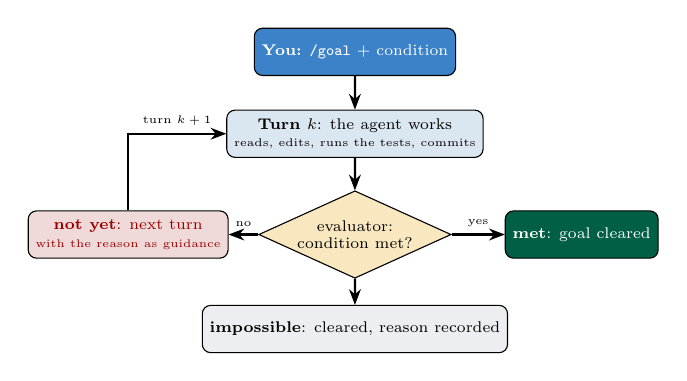
\begin{tikzpicture}[
    box/.style={draw, rounded corners=3pt, minimum width=3.0cm, minimum height=0.75cm, font=\scriptsize, align=center},
    dec/.style={draw, diamond, aspect=2.2, fill=softorange!25, font=\scriptsize, align=center, inner sep=1pt},
    arr/.style={-{Stealth[length=2mm]}, thick}, scale=0.8, transform shape]
    \node[box, fill=level4, text=white] (you) at (0,3.2) {\textbf{You:} \texttt{/goal} + condition};
    \node[box, fill=softblue!20] (turn) at (0,1.9) {\textbf{Turn $k$}: the agent works\\{\tiny reads, edits, runs the tests, commits}};
    \node[dec] (q) at (0,0.3) {evaluator:\\condition met?};
    \node[box, fill=softgreen!60!black, text=white, minimum width=2.4cm] (done) at (3.6,0.3) {\textbf{met}: goal cleared};
    \node[box, fill=harvardcrimson!15, text=harvardcrimson, minimum width=2.4cm] (no) at (-3.6,0.3) {\textbf{not yet}: next turn\\{\tiny with the reason as guidance}};
    \node[box, fill=uzhgreylight, minimum width=2.4cm] (imp) at (0,-1.2) {\textbf{impossible}: cleared, reason recorded};
    \draw[arr] (you) -- (turn); \draw[arr] (turn) -- (q);
    \draw[arr] (q) -- node[above, font=\tiny] {yes} (done);
    \draw[arr] (q) -- node[above, font=\tiny] {no} (no);
    \draw[arr] (q) -- (imp);
    \draw[arr] (no.north) |- node[pos=0.75, above, font=\tiny] {turn $k+1$} (turn.west);
\end{tikzpicture}
\end{center}
\column{0.42\textwidth}
\begin{lstlisting}[style=bash, basicstyle=\scriptsize\ttfamily]
# set: the first turn starts at once
/goal all tests pass: `pytest -q`
      exits 0. Or stop after 6 turns.
/goal          # status: turns, time, spend
/goal clear    # end it yourself
claude -p "/goal <condition>"  # headless
\end{lstlisting}
\vspace{0.3em}
\textbf{A condition that holds up}
\begin{itemize}\itemsep2pt
  \item one measurable end state and the command that proves it
  \item constraints that must hold on the way
  \item a bound: ``or stop after 6 turns''
\end{itemize}
\vspace{0.3em}
The evaluator reads only the transcript, so the agent must \emph{show} the test output. Permissions are unchanged: allow the test command, or run in auto mode.
\end{columns}
\end{frame}

% --- The demo problem ---
\begin{frame}{What a Deep Equilibrium Net Is}
\footnotesize
\hfill\stepmarker{4}
Azinovic, Gaegauf and Scheidegger (2022, \emph{IER}): solve a dynamic model by training a neural network to satisfy its equilibrium conditions.
\begin{columns}[T]
\column{0.50\textwidth}
\begin{enumerate}\itemsep4pt
  \item \textbf{The unknown is a function.} The policy, here the savings rate $s(z, K)$, is represented by a small network $s_\theta(x)$ with $x = (\log z/\mathrm{sd}_z,\ \log K - \log K^*)$ and a sigmoid output, so $s \in (0, 1)$.
  \item \textbf{The equilibrium condition is the loss.} At a batch of states the Euler residual $r(x)$ is computed, the expectation by five quadrature nodes; $\theta$ moves by gradient descent on the mean of $r^2$, derivatives by automatic differentiation.
  \item \textbf{No grid.} The paper draws the training states by simulating the network's own policy, so the solution is accurate where the economy lives, and the method scales to many state variables. Today's version draws them from a fixed box around $K^*$; the on-path check of Step 3 restores the paper's criterion.
\end{enumerate}
\column{0.46\textwidth}
\begin{block}{The residual, a fraction of consumption}
\[
r(x) = \beta\, C\, \mathbb{E}\!\left[\frac{1-\delta+\alpha z' K'^{\alpha-1}}{C'}\right] - 1
\]
zero at the solution; the tests ask how far from zero, where the policy sends the economy, and how far the policy is from the reference solver.
\end{block}
\vspace{0.3em}
\textbf{Why this problem for a loop demo:} a known answer at the same states, a way to be wrong that \emph{looks} right (Part VIII), and eleven seconds per training run on a laptop.
\end{columns}
\filebox{Azinovic, Gaegauf \& Scheidegger (2022), International Economic Review 63(4); code/deqn/README.md}
\end{frame}

\begin{frame}[fragile]{The Residual, as the Reference Solution Writes It}
\footnotesize
\begin{columns}[T]
\column{0.60\textwidth}
\begin{lstlisting}[basicstyle=\scriptsize\ttfamily]
def residual(net, logz, logK):
    z, K = torch.exp(logz), torch.exp(logK)
    Y = z * K ** ALPHA
    x = common.encode_state(logz, logK, P)
    s = net(x).squeeze(1)
    C = (1.0 - s) * Y
    Kn = (1.0 - DELTA) * K + s * Y
    logKn = torch.log(Kn)
    E = torch.zeros_like(C)
    for e, w in zip(NODES, WEIGHTS):
        logzn = RHO * logz + SIGMA * e
        zn = torch.exp(logzn)
        xn = common.encode_state(logzn, logKn, P)
        sn = net(xn).squeeze(1)
        Cn = (1.0 - sn) * zn * Kn ** ALPHA
        Rn = 1.0 - DELTA + ALPHA * zn * Kn ** (ALPHA - 1.0)
        E = E + w * Rn / Cn
    return BETA * C * E - 1.0
\end{lstlisting}
\column{0.38\textwidth}
\textbf{Sixteen lines} (lightly reformatted here): today's consumption, tomorrow's capital, the expectation over five shocks, the gap.

\vspace{0.5em}
\textbf{The training loop} is twelve more: seed torch, \texttt{make\_net(2, s\_init=s*)}, Adam, and 2,000 times: draw 128 states, \texttt{loss = (residual(...) ** 2).mean()}, backward, step.

\vspace{0.5em}
\textbf{The agent writes all of it} from the goal on the next slides; the reference solution stays outside the demo project.
\end{columns}
\filebox{code/deqn/solution/deqn\_stochastic.py (96 lines); the shared pieces: code/deqn/common.py}
\end{frame}

% --- Live: the loop ---
\begin{frame}[fragile]{\walkthrough~6: The Tests Are the Spec~\livedemo}
\footnotesize
\hfill\stepmarker{4}
\begin{columns}[T]
\column{0.56\textwidth}
\texttt{tests/test\_deqn\_stochastic.py}, abridged (the stub it tests raises \texttt{NotImplementedError}):
\begin{lstlisting}[basicstyle=\scriptsize\ttfamily, frame=single, rulecolor=\color{uzhgreydark!40}]
from deqn.stochastic import solve
MEAN_ABS_RESIDUAL = 1e-3   # reference: 1.4e-4
MAX_POLICY_GAP = 1e-2      # reference: 2.3e-3

def test_residual_on_own_path(trained, path):
    LZ, LK = path
    r = euler_residual(trained["s"], LZ, LK)
    assert np.abs(r).mean() < MEAN_ABS_RESIDUAL

def test_policy_matches_reference(trained):
    ref = np.loadtxt(REFERENCE_CSV, ...)
    s_net = trained["s"](ref[:, 0], ref[:, 1])
    gap = np.abs(s_net - ref[:, 2]).max()
    assert gap < MAX_POLICY_GAP

# + mean savings rate, path inside the window,
#   same seed -> same policy
\end{lstlisting}
\column{0.42\textwidth}
\textbf{Where the thresholds come from}
\begin{center}
\scriptsize
\renewcommand{\arraystretch}{1.2}
\begin{tabular}{@{}lrr@{}}
\toprule
 & \textbf{reference} & \textbf{threshold} \\
\midrule
on-path mean $|r|$ & 1.4e-4 & $< 10^{-3}$ \\
max $|s - s_{\mathrm{ref}}|$ & 2.3e-3 & $< 10^{-2}$ \\
$|E[s] - 0.2521|$ & 2e-4 & $< 5\cdot10^{-3}$ \\
own-path $\log K$ in window & yes & always \\
two runs, same seed & identical & equality \\
\bottomrule
\end{tabular}
\end{center}
\vspace{0.2em}
4--25$\times$ what the reference solution reaches. The tests' own residual and simulation live in \texttt{conftest.py}, independent of the solver, so the agent cannot talk its way past them.
\end{columns}
\filebox{code/deqn/tests/, code/deqn/reference/baseline.md (the measured run and every margin); the solution kept apart: code/deqn/solution/}
\end{frame}

% --- Anatomy of the goal ---
\begin{frame}[fragile]{The Goal, Taken Apart~\livedemo}
\footnotesize
\hfill\stepmarker{4}
Typed in a second terminal, in the demo project, at the start of this part. Six parts; each answers a question the agent would otherwise guess anew every turn.
\begin{lstlisting}[style=prompt, basicstyle=\scriptsize\ttfamily]
(*@\textcolor{level5}{\textbf{[CONDITION]}}@*) /goal `python3 -m pytest -q tests/` in this project exits 0 with 5 passed.
(*@\textcolor{softblue}{\textbf{[PROBLEM]}}@*)   To get there, implement solve(seed, steps) in deqn/stochastic.py: a DEQN for
             the stochastic growth model of CLAUDE.md.
(*@\textcolor{softgreen!80!black}{\textbf{[RECIPE]}}@*)    State via common.encode_state; network common.make_net(2, s_init=s*); loss =
             mean squared Euler residual with common.gh_nodes(5); 128 fresh states per
             step; Adam 1e-3, 2000 steps, torch.manual_seed(seed) first, float64.
(*@\textcolor{softorange!90!black}{\textbf{[INTERFACE]}}@*) solve returns {"s": callable (log_z, log_K) -> savings rate, numpy in and
             out, "net", "wall"} and saves results/deqn_stochastic.pt via save_policy.
(*@\textcolor{darkred}{\textbf{[EACH TURN]}}@*) Run the tests and show the output, fix one thing, commit. Never edit tests/
             or reference/. Report ALL_TESTS_PASS when pytest exits 0.
(*@\textcolor{harvardcrimson}{\textbf{[CAP]}}@*)       Stop after 6 turns (count your commits) and write notes/blocked.md instead.
\end{lstlisting}
\vspace{0.2em}
\begin{center}
\renewcommand{\arraystretch}{1.15}
\begin{tabular}{@{}l p{10.6cm}@{}}
\textcolor{level5}{\textbf{Condition}} & what ``done'' means, readable off the transcript by the evaluator \\
\textcolor{softblue}{\textbf{Problem}} & the model and where it is stated, so turn 1 does not guess the equation \\
\textcolor{softgreen!80!black}{\textbf{Recipe}} & a reproducible eleven-second run: the Step-2 prompt again \\
\textcolor{softorange!90!black}{\textbf{Interface}} & the function the tests import; a mismatch fails for the wrong reason \\
\textcolor{darkred}{\textbf{Each turn}} & verifier first, output shown, one fix, one commit; the exam is off limits \\
\textcolor{harvardcrimson}{\textbf{Cap}} & bound the cost; say how to count; say what to do when stuck \\
\end{tabular}
\end{center}
\filebox{code/prompts.md, \S 11 (the goal verbatim, and a template with the six parts as placeholders for your own project)}
\end{frame}

% --- Turn by turn ---
\begin{frame}[fragile]{The Loop, Turn by Turn}
\footnotesize
\hfill\stepmarker{4}
The second terminal (an illustrative transcript, condensed; your run differs in detail).
\begin{columns}[T]
\column{0.58\textwidth}
\begin{lstlisting}[style=bash, basicstyle=\scriptsize\ttfamily]
--- turn 1 ---
[Read tests/, deqn/common.py, CLAUDE.md]
[Write deqn/stochastic.py]  residual, loop, solve()
[Bash pytest -q tests/]  .FF.F  3 failed, 2 passed
   TypeError in the oracle: s() returned a
   tensor, the tests expect numpy arrays
[Bash git commit -m "turn 1: DEQN solver"]
  evaluator: NOT YET MET -> turn 2

--- turn 2 ---
[Edit deqn/stochastic.py]  s(): no_grad, .numpy()
[Bash pytest -q tests/]  .....  5 passed  (14 s)
[Bash git commit -m "turn 2: 5 passed"]
ALL_TESTS_PASS  mean |r| 1.4e-4, E[s] 0.2523
  evaluator: MET. 2 turns, 1 min 30 s.
\end{lstlisting}
\column{0.40\textwidth}
\begin{center}
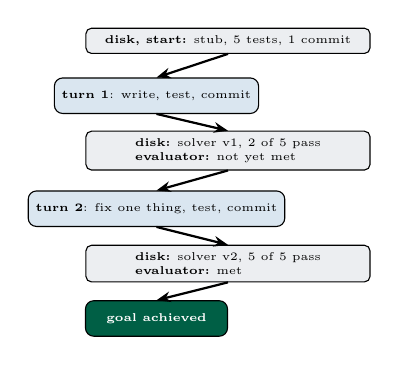
\begin{tikzpicture}[
    st/.style={draw, rounded corners=2pt, fill=uzhgreylight, font=\tiny, align=left, minimum width=4.4cm, anchor=west},
    it/.style={draw, rounded corners=3pt, font=\tiny, align=center, minimum width=2.2cm, minimum height=0.55cm},
    arr/.style={-{Stealth[length=1.8mm]}, thick}, scale=0.82, transform shape]
    \node[st] (d0) at (0,3.3) {\textbf{disk, start:} stub, 5 tests, 1 commit};
    \node[it, fill=softblue!20] (i1) at (1.1,2.45) {\textbf{turn 1}: write, test, commit};
    \node[st] (d1) at (0,1.6) {\textbf{disk:} solver v1, 2 of 5 pass\\\textbf{evaluator:} not yet met};
    \node[it, fill=softblue!20] (i2) at (1.1,0.7) {\textbf{turn 2}: fix one thing, test, commit};
    \node[st] (d2) at (0,-0.15) {\textbf{disk:} solver v2, 5 of 5 pass\\\textbf{evaluator:} met};
    \node[it, fill=softgreen!60!black, text=white] (end) at (1.1,-1.0) {\textbf{goal achieved}};
    \draw[arr] (d0.south) -- (i1.north); \draw[arr] (i1.south) -- (d1.north);
    \draw[arr] (d1.south) -- (i2.north); \draw[arr] (i2.south) -- (d2.north);
    \draw[arr] (d2.south) -- (end.north);
\end{tikzpicture}
\end{center}
\textbf{What to notice:} a \emph{different} model decides completion; the failures named a format mismatch, not an economics error; one fix, and the on-path checks passed.
\end{columns}
\filebox{afterwards, in the demo project: python3 -m pytest -q tests/, git log --oneline, /goal, then /deqn-accuracy results/deqn\_stochastic.pt}
\end{frame}

% --- The verification figure ---
\begin{frame}[fragile]{After the Loop: Three Panels That Confirm the Solution}
\footnotesize
\hfill\stepmarker{4}
Five passed tests are numbers. The \texttt{/deqn-accuracy} skill (\texttt{accuracy.py -{}-plot}) draws the same checks for the policy the \texttt{/goal} built, so that ``solved'' is something you can see:
\begin{center}
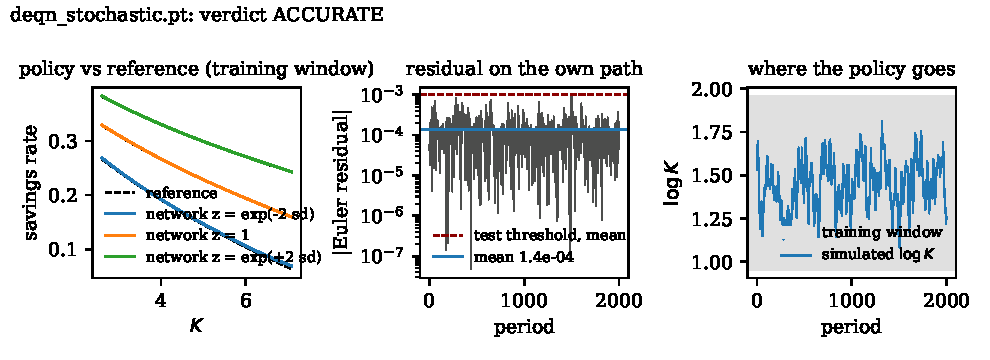
\includegraphics[width=0.8\linewidth]{figures/agentic_deqn_verify_good.pdf}
\end{center}
\vspace{-0.3em}
\begin{columns}[T]
\column{0.31\textwidth}
\textbf{The right policy.} The network (solid) lies on the reference solver (dashed) across the training window, at low, average and high productivity.
\column{0.31\textwidth}
\textbf{The equation holds.} The Euler residual along 2,000 simulated periods: mean $1.4\times10^{-4}$, a tenth of the test threshold, nowhere blowing up.
\column{0.31\textwidth}
\textbf{Checked where it matters.} Capital under the network's own policy stays inside the training window: the other panels were evaluated where the economy lives.
\end{columns}
\filebox{code/deqn/accuracy.py (-{}-plot); slides/figures/agentic\_deqn\_verify\_good.pdf}
\end{frame}

% --- Guardrails + headless ---
\begin{frame}{Guardrails for a Closed Loop}
\footnotesize
\textbf{Hard prerequisites}
\begin{enumerate}\itemsep4pt
  \item \emphc{Verifier or no goal.} If you cannot write a command that exits 0 when, and only when, the task is done, do not close the loop on it.
  \item \emphc{Tight conditions.} ``\texttt{estimate.py} reports cluster-robust SEs and the tests pass'': yes. ``Replicate Acemoglu, Johnson and Robinson (2001)'': no.
  \item \emphc{Cost cap} in the condition: ``or stop after 6 turns''; \texttt{/goal} shows the spend so far.
  \item \emphc{Rules on.} Deny rules on the confidential folders, the \texttt{PreToolUse} guard, \texttt{CLAUDE.md} read-only paths (Part VI).
  \item \emphc{Throw-away branch.} Review the result like a pull request from a junior colleague: \texttt{git diff main...HEAD}, then merge or discard.
\end{enumerate}

\vspace{0.6em}
\begin{alertblock}{Two failure modes to expect}
\textbf{Compounding errors:} a wrong assumption in turn 2 propagates to turns 3--6; the evaluator checks the condition, not the economics. Short loops, frequent diff review.\\[3pt]
\textbf{Token blow-up:} a turn that re-runs a test suite and edits a file costs roughly \$0.50--1 on Opus; six turns are a few dollars, sixty are not. Cap it.
\end{alertblock}
\end{frame}

\begin{frame}[fragile]{Running Without a Terminal}
\footnotesize
\begin{columns}[T]
\column{0.58\textwidth}
\textbf{Headless: the same agent in a batch job}
\begin{lstlisting}[style=bash, basicstyle=\scriptsize\ttfamily]
# print mode: no UI; cron or Slurm
claude -p "Re-run estimate.py on
  the new data, refresh tables/,
  log the changes" \
  --allowedTools "Read,Edit,Bash"

# a goal, headless
claude -p "/goal pytest -q exits 0"

# fresh context per run (Ralph):
# your test decides; disk remembers
while ! pytest -q tests/; do
  claude -p "$(cat PROMPT.md)"
done
\end{lstlisting}
\column{0.40\textwidth}
\begin{center}
\renewcommand{\arraystretch}{1.25}
\begin{tabular}{p{2.3cm} p{2.6cm}}
\toprule
\textbf{Need} & \textbf{Tool} \\
\midrule
Interactive work & \texttt{claude}, \texttt{/goal} \\
Scheduled, one prompt & \texttt{claude -p} in cron / Slurm \\
Your own harness & Agent SDK (Python, TypeScript) \\
Hosted, long-running & Managed Agents \\
\bottomrule
\end{tabular}
\end{center}
\vspace{0.3em}
Same permissions, same hooks, same \texttt{CLAUDE.md}. A headless run on confidential data has exactly the governance problem of Part IX, with nobody watching.
\end{columns}
\filebox{code/prompts.md, \S 12 (the headless commands and the shell loop); docs: code.claude.com/docs/en/agent-sdk/overview}
\end{frame}

% ============================================================================
% PART VIII: FROM PLAN TO PAPER SECTION
% ============================================================================
\partcard{VIII}{From Plan to Table and Figure}

% --- Walk-through 7: the plan ---
\begin{frame}[fragile]{\walkthrough~7: The Plan, and How It Was Reconciled}
\footnotesize
\hfill\stepmarker{5}
Step 4 in plan mode instead of as a goal: the plan, written from the course notebook's recipe before any code, and what the run did to it.
\begin{columns}[T]
\column{0.49\textwidth}
\begin{lstlisting}[style=md, basicstyle=\scriptsize\ttfamily]
## Problem
Loss: r = beta C E[...] - 1. Known answer:
brock_mirman_reference.solve(0.96, 0.9).
## Recipe
- x = (log z / sd_z, log K - log K*)
- 2-32-32-1 tanh, sigmoid (notebook init)
- 5 GH nodes; 128 fresh states per step
- Adam 1e-3, 2000 steps, seed 42, float64
## Targets (reference/baseline.md)
| mean |r| on the own path     | < 1e-3 |
| max |s - s_ref|              | < 1e-2 |
| |E[s] - 0.2521|              | < 5e-3 |
| own-path log K in the window | always |
\end{lstlisting}
The reference and the four targets were in the plan \emph{before any code}.
\column{0.49\textwidth}
\begin{lstlisting}[style=md, basicstyle=\scriptsize\ttfamily]
## First implementation: as planned
Loss 2.9e-7, the lowest of any run. On-path
mean |r| 9.2e-2; E[s] 0.94 instead of 0.25;
log K drifted to [3.14, 3.72], outside the
box. WRONG on four of five tests.
## Revised recipe (achieved)
One change: s_init = s*. Loss 6.0e-7 (higher);
mean |r| 1.4e-4; max |s - s_ref| 2.3e-3;
E[s] 0.2523; log K in [1.08, 1.81]. All pass.
## Sanity rule
The constant policy s = s* gives |r| = 1.2e-2.
A smaller RMS residual far from s* is a
wrong branch, not a solution.
\end{lstlisting}
\textbf{Why this step matters:} the target was not met at first, and nothing in the training loop said so. The difference between the two versions is the finding: next slide.
\end{columns}
\filebox{code/deqn/plan\_deqn.md (written for the lecture; the numbers are measured); the two runs: solution/deqn\_stochastic.py, stochastic\_box.py}
\end{frame}

% --- The silent failure ---
\begin{frame}[fragile]{The Silent Failure: A Loss That Converged, a Policy That Did Not}
\footnotesize
\hfill\stepmarker{6}
\begin{columns}[T]
\column{0.49\textwidth}
\centering
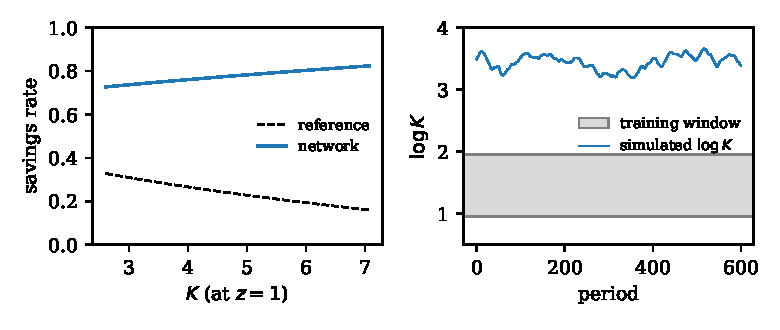
\includegraphics[width=0.88\linewidth]{figures/agentic_deqn_silent_bad.pdf}\\
{\scriptsize \textbf{The notebook's recipe:} loss $2.9\times10^{-7}$; savings rate 0.94; the economy leaves the box.}
\column{0.49\textwidth}
\centering
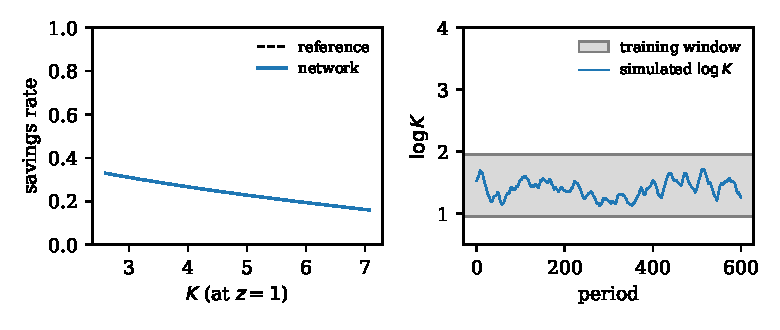
\includegraphics[width=0.88\linewidth]{figures/agentic_deqn_silent_good.pdf}\\
{\scriptsize \textbf{One line changed} (\texttt{s\_init=s*}): loss $6.0\times10^{-7}$, \emph{higher}; the policy sits on the reference.}
\end{columns}

\vspace{0.4em}
\begin{columns}[T]
\column{0.50\textwidth}
\renewcommand{\arraystretch}{1.15}
\begin{tabular}{@{}lrr@{}}
\toprule
 & \textbf{notebook recipe} & \textbf{with \texttt{s\_init}} \\
\midrule
training loss & $2.9\times10^{-7}$ & $6.0\times10^{-7}$ \\
on-path mean $|r|$ & $9.2\times10^{-2}$ & $1.4\times10^{-4}$ \\
$E[s]$ (reference 0.252) & 0.937 & 0.252 \\
$\log K$ (box $[0.96, 1.96]$) & $[3.14, 3.72]$ & $[1.08, 1.81]$ \\
\bottomrule
\end{tabular}
\column{0.47\textwidth}
\begin{alertblock}{The lesson}
The Euler equation is \emph{necessary}, not sufficient: it also has an over-saving branch ($s$ rising in $K$, $C \to 0$) that transversality rules out and the loss does not. The initialisation picks the branch. What caught it: the network's own path, four of the five tests.
\end{alertblock}
\end{columns}
\filebox{code/deqn/silent\_failure.md, stochastic\_box.py (the one-line diff: s\_init=None), plot\_silent\_failure.py (redraws both figures)}
\end{frame}

% --- One prompt -> table + figure ---
\begin{frame}[fragile]{One Prompt $\to$ Table $+$ Figure~\livedemo}
\footnotesize
\hfill\stepmarker{7}
Does the loss kernel matter? One prompt settles it, with the accuracy measure we trust.
\begin{columns}[T]
\column{0.46\textwidth}
\begin{lstlisting}[style=prompt, basicstyle=\scriptsize\ttfamily]
> Role: computational macroeconomist.
  Task: train deqn/stochastic.py four
  times, only the loss kernel changed:
  MSE, MAE, Huber, log-cosh; seed 42.
  Evaluate each on its own simulated
  path: |residual| mean, p99, max;
  E[s]; max |s - s_ref|.
  Outputs: deqn_kernel_table.tex
  (booktabs), deqn_kernel_figure.pdf.
  Do NOT modify common.py or tests/.
  Verify: every E[s] within 5e-3.
\end{lstlisting}
\column{0.52\textwidth}
\begin{center}
\scriptsize
\renewcommand{\arraystretch}{1.1}
\begin{tabular}{lrrrr}
\toprule
Kernel & train.\ loss & mean $|r|$ & $E[s]$ & max $|s - s_{\mathrm{ref}}|$ \\
\midrule
MSE & 6.0e-07 & 1.4e-04 & 0.2523 & 2.3e-03 \\
MAE & 2.9e-04 & 1.7e-04 & 0.2520 & 1.4e-03 \\
Huber & 2.0e-07 & 9.9e-05 & 0.2521 & 2.0e-03 \\
log-cosh & 3.0e-07 & 1.4e-04 & 0.2523 & 2.3e-03 \\
\bottomrule
\end{tabular}
\end{center}
\begin{center}
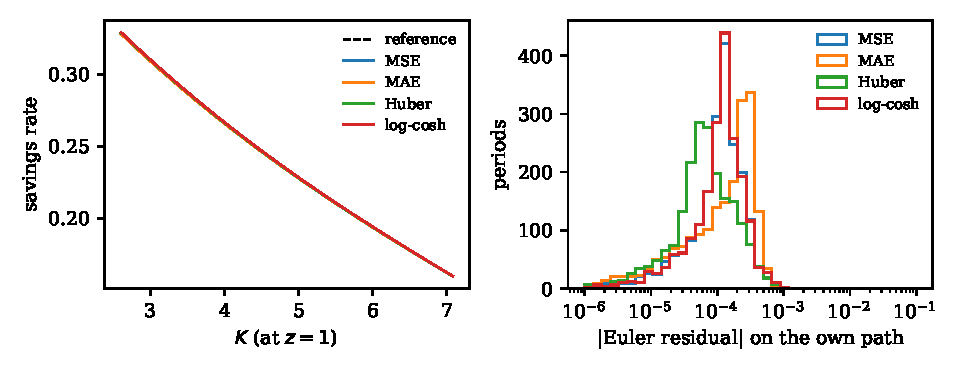
\includegraphics[width=0.7\linewidth]{figures/agentic_deqn_kernels.pdf}
\end{center}
The training-loss column cannot rank them: its rows are in different units (MAE in $|r|$, the rest in $r^2$). On the path all four agree to $3\times10^{-4}$; only those columns can say so.
\end{columns}
\filebox{code/deqn/loss\_kernels.py (92 lines, 35 s), outputs/deqn\_kernel\_table.tex (three columns omitted here); prompt: code/prompts.md, \S 13}
\end{frame}

% --- Full pipeline ---
\begin{frame}{The Full Research Pipeline}
\footnotesize
\hfill\stepmarker{7}
\begin{center}

\begin{tikzpicture}[
    pst/.style={draw, rounded corners=3pt, minimum width=1.9cm, minimum height=0.8cm, font=\scriptsize\bfseries, align=center, text=white},
    lab/.style={font=\tiny\ttfamily, text=uzhgreydark, align=center},
    arr/.style={-{Stealth[length=2mm]}, thick, uzhblue}, scale=0.95, transform shape]
    \node[pst, fill=level5] (raw) at (0,0) {Observed\\panel};
    \node[pst, fill=level4] (mom) at (2.5,0) {Moments};
    \node[pst, fill=level3] (est) at (5.0,0) {Estimates\\$\hat\varrho$};
    \node[pst, fill=softblue!80!black] (deqn) at (7.5,0) {DEQN at $\hat\varrho$\\verdict};
    \node[pst, fill=softorange!80!black] (out) at (10.0,0) {Figures,\\tables};
    \node[pst, fill=harvardcrimson] (paper) at (12.5,0) {Paper\\section};
    \foreach \a/\b/\t in {raw/mom/moments.py, mom/est/estimate\_rho.py, est/deqn/check\_deqn.py, deqn/out/make\_table.py, out/paper/verify.py} {\draw[arr] (\a) -- (\b); \node[lab] at ($(\a)!0.5!(\b)+(0,0.65)$) {\t};}
\end{tikzpicture}
\end{center}
\vspace{0.3em}
\textbf{Six prompts, one per step}, each a Level-3 prompt producing a file the next step reads:
\begin{enumerate}\itemsep2pt
  \item \textbf{Diagnostics:} ``Read \texttt{data/bm\_panel.csv}. Do NOT read the truth file.'' (or \texttt{/data-diagnostics})
  \item \textbf{Moments} per economy to JSON, with \texttt{bm.moments}, not re-implemented
  \item \textbf{Estimate $\varrho$} by simulated method of moments, the reference solver in the loop; common random numbers, fixed seeds
  \item \textbf{The solver we built, at $\hat\varrho$:} train \texttt{deqn/stochastic.py} at $\hat\varrho$, \texttt{/deqn-accuracy} against \texttt{solve(0.96, rho\_hat)}
  \item \textbf{Figures and tables:} criterion per economy; a booktabs table of $\hat\varrho$, data vs fitted moments, DEQN verdict
  \item \textbf{Verify, then draft:} ``Now read the truth file: $|\hat\varrho - \varrho| < 0.05$?'' Then 300 words, every number traced to a file
\end{enumerate}
\vspace{0.2em}
\texttt{run\_all.py} chains the steps; the truth is read once, in \texttt{verify.py}, after the table is written.
\filebox{code/prompts.md, \S 14 (all six prompts and run\_all.py)}
\end{frame}

% --- Replication ---
\begin{frame}[fragile]{AI Agents for Paper Replication}
\footnotesize
\begin{columns}[T]
\column{0.48\textwidth}
\textbf{Why replication is the best training ground}
\begin{itemize}\itemsep3pt
  \item A bounded task with a \emphc{clear success criterion}: do the numbers match?
  \item It forces every skill above: plan, constrain, verify, document
  \item A genuine contribution, and the starting point for extending a method
\end{itemize}
\vspace{0.4em}
\textbf{The replication ladder}
\begin{center}
\renewcommand{\arraystretch}{1.2}
\begin{tabular}{p{3.4cm} l}
\toprule
\textbf{Paper type} & \textbf{Agent success} \\
\midrule
Documented, code available & \textcolor{darkgreen}{\textbf{High}} \\
Documented, no code & \textcolor{softorange}{\textbf{Moderate}} \\
Sparse, standard method & \textcolor{softorange}{\textbf{Moderate}} \\
Novel method & \textcolor{darkred}{\textbf{Low}} \\
\bottomrule
\end{tabular}
\end{center}
\column{0.48\textwidth}
\textbf{The replication prompt}
\begin{lstlisting}[style=prompt, basicstyle=\scriptsize\ttfamily]
> Role: replication engineer.
  Paper: [title, authors, DOI]
  Mission: replicate ALL figures and
  tables.
  1. Do NOT use the authors' code
  2. Track progress in notes/todo.md
  3. Commit after each step
  4. Stuck x3: notes/blocked.md, STOP
  First: the figures' axes and CIs,
  then notes/plan.md; wait.
  Final: "paper value vs our value"
\end{lstlisting}
\vspace{0.2em}
\textbf{Verification:} within one standard error of the paper's value is a match. The table of mismatches is the research question.
\end{columns}
\filebox{code/prompts.md, \S 15}
\end{frame}

% ============================================================================
% PART IX: VERIFICATION, REPRODUCIBILITY, GOVERNANCE
% ============================================================================
\partcard{IX}{Verification, Reproducibility \& Governance}

% --- Cardinal rule ---
\begin{frame}{The Cardinal Rule: Never Skip Verification}
\footnotesize
\begin{alertblock}{The invisible failure mode}
Code that \emphc{crashes} is visible. Code that runs cleanly, reports the best loss of any run and returns a savings rate of 0.94 instead of 0.25 (Part VIII) is \emphc{invisible}: the agent's characteristic failure.
\end{alertblock}

\vspace{0.4em}
\begin{columns}[T]
\column{0.48\textwidth}
\textbf{Four verification steps, every time}
\begin{enumerate}\itemsep4pt
  \item \textbf{Known-answer test.} Simulate at $\varrho = 0.9$, estimate: $\hat\varrho \approx 0.9$? A staggered-adoption panel with a true effect of 0.10: does your code recover it?
  \item \textbf{Reproduce a stored result} before changing anything.
  \item \textbf{Check the solution, not the loss.} The policy against the reference, on the path the policy itself generates; the coefficient against the paper.
  \item \textbf{Simple-case limit.} The closed form at $\delta = 1$; the truth at $N = 10^5$.
\end{enumerate}
\column{0.48\textwidth}
\textbf{Five things agents get wrong}, each worth a constraint or a test:

\vspace{0.3em}
\textbf{scales} (one loss term or moment silently dominates), \textbf{samples} (a box instead of the ergodic set, the wrong estimation window), \textbf{constraints} (a penalty where a complementarity condition was needed), \textbf{standard errors and timing} (the wrong cluster level, two-way fixed effects on staggered adoption), \textbf{identification} (a flat criterion blamed on the optimiser, or the reverse).

\vspace{0.4em}
The fixes are the failure-mode table of Part IV and the tests of Part VII.
\end{columns}
\end{frame}

% --- Disclosure ---
\begin{frame}{Disclosure Norms by Publisher (2023--2026)}
\footnotesize
A snapshot; check the \emph{specific} journal before submission and before refereeing.
\begin{center}
\renewcommand{\arraystretch}{1.1}
\begin{tabular}{p{2.8cm} p{5.6cm} p{3.6cm}}
\toprule
\textbf{Publisher} & \textbf{Authors} & \textbf{Referees} \\
\midrule
AEA journals & describe AI use at submission; authors accountable & check the current policy \\
\textit{QJE}, \textit{JPE}, \textit{REStud}, \textit{Econometrica} & disclose substantive use; authors responsible for all content & check the reviewer guidelines \\
Elsevier (\textit{JME}, \textit{JPubE}) & statement at the end of the manuscript; no AI images & must not upload the manuscript to an AI tool \\
Springer Nature, \textit{Science} & document use in Methods or the cover letter & AI use in review not permitted \\
COPE (2023) & ``AI tools cannot meet the requirements for authorship'' & confidentiality applies \\
\bottomrule
\end{tabular}
\end{center}

\vspace{0.3em}
\begin{alertblock}{Bottom line}
Any use that produced a number, a figure, a derivation or more than a sentence of text is disclosable: model, version, date, and a prompt log next to the replication package.
\end{alertblock}
\textbf{A model sentence:} {\itshape ``The code in Sections 3--4 was drafted with Claude Code (Opus 5.5, November 2026) from the prompts in \texttt{replication/prompts.md}; all results were verified by the authors.''}
\end{frame}

% --- Referees, supervisors, students ---
\begin{frame}{What This Means for Referees, Supervisors and Students}
\footnotesize
\begin{columns}[T]
\column{0.49\textwidth}
\begin{block}{As a referee or editor}
\begin{itemize}\itemsep3pt
  \item The manuscript is confidential; an LLM is a third party. Most publishers prohibit uploading a submission.
  \item An agent on \emph{your own} notes about the paper is different; say so, and let the editor decide.
\end{itemize}
\end{block}
\begin{block}{As a supervisor}
\begin{itemize}\itemsep3pt
  \item The faculty's integrity rules apply. Agree the disclosure with the student \emph{before} the work starts.
  \item The student must be able to explain every line the agent wrote. Ask for the verification, not the code.
\end{itemize}
\end{block}
\column{0.49\textwidth}
\begin{block}{As a PhD student}
\begin{itemize}\itemsep3pt
  \item Keep the transcripts (\texttt{\textasciitilde/.claude/projects/}; \texttt{/export}), or at least a \texttt{prompts.md} with model, version and date.
  \item ``Is it still my work?'' The standard is the RA's code: you specified it, you verified it, you can defend every line.
\end{itemize}
\end{block}
\end{columns}

\vspace{0.3em}
\textbf{Three rules that do not change:} you are accountable for every number; confidential material does not go to a third party; disclosure is cheap, discovery is not.
\end{frame}

% --- Replication packages ---
\begin{frame}[fragile]{Replication Packages in the Age of LLMs}
\footnotesize
\begin{columns}[T]
\column{0.52\textwidth}
\textbf{The new failure mode.} An LLM call is \emph{non-deterministic}. Re-running an analysis no longer means identical numbers, unless the LLM output is frozen as code and checked in.

\vspace{0.4em}
\textbf{What the AEA Data Editor's rules, read literally, imply}
\begin{enumerate}\itemsep2pt
  \item Every artifact re-runnable \emph{without} re-querying any LLM
  \item Data lineage (raw $\to$ processed $\to$ tables) fully scripted
  \item Random seeds pinned and documented
\end{enumerate}

\vspace{0.4em}
\textbf{What to ship}
\begin{itemize}\itemsep2pt
  \item All code, LLM-generated code included, as \emphc{frozen} files
  \item A lockfile, and a container image where feasible
  \item \texttt{prompts.md}: model, version and date for every artifact
  \item \texttt{CLAUDE.md}, sensitive-path rules redacted
\end{itemize}
\column{0.45\textwidth}
\begin{alertblock}{Anti-patterns}
\begin{itemize}\itemsep2pt
  \item ``Re-run \texttt{claude} on \texttt{prompt.md}.'' \emph{Will not reproduce.}
  \item An LLM call inside \texttt{run\_all.py} without a pinned model and version
  \item Auto-commit messages as the only documentation
\end{itemize}
\end{alertblock}
\vspace{0.3em}
\textbf{Hallucinated citations}
\begin{lstlisting}[style=prompt, basicstyle=\scriptsize\ttfamily]
> Do NOT invent citations. Only cite
  references.bib. If unsure:
  [CITE: author, year -- verify]
\end{lstlisting}
Walters \& Wilder (2023): 55\,\% of GPT-3.5 citations were fabricated. The real fix is retrieval (a Zotero MCP server), not an instruction.
\end{columns}
\end{frame}

% --- Governance ---
\begin{frame}{Data Governance: GDPR, the EU AI Act, Data Agreements}
\footnotesize
Everything the agent \emph{reads} goes into the API call. With licensed or confidential research data, this question comes first.

\vspace{0.4em}
\begin{columns}[T]
\column{0.50\textwidth}
\textbf{Three regimes that apply}
\begin{itemize}\itemsep4pt
  \item \emphc{GDPR}: personal data to a US-hosted API needs a lawful basis, a processor agreement (API, Team and Enterprise contracts; not consumer plans) and a transfer mechanism.
  \item \emphc{Research-data agreements}: restricted microdata are confidential by contract, whatever the cloud contract says.
  \item \emphc{EU AI Act}: duties fall mainly on model providers; deployers have transparency duties (Art.\ 50).
\end{itemize}
\column{0.47\textwidth}
\textbf{Practical defaults}
\begin{itemize}\itemsep4pt
  \item[\textcolor{darkred}{\ding{55}}] Confidential, granular or personal data, credentials: never to a public API
  \item[\textcolor{softorange}{\textbf{?}}] Licensed or DUA data: re-read the agreement first
  \item[\textcolor{darkgreen}{\checkmark}] Public data, synthetic data, model code: fine; send the aggregate or the synthetic twin
  \item[\textcolor{darkgreen}{\checkmark}] Deny rules, the hook, read-only paths: none airtight; restricted data stays on a machine the agent does not run on
\end{itemize}
\end{columns}

\vspace{0.5em}
\textbf{The institutional route:} Claude Code against Amazon Bedrock, Google Cloud or Microsoft Foundry in your own tenancy; zero data retention for qualified Enterprise accounts. A question for IT and legal, not for a laptop.
\end{frame}

% --- Six habits ---
\begin{frame}{Six Habits That Make Compliance Checkable}
\footnotesize
\begin{columns}[T]
\column{0.60\textwidth}
\begin{block}{Six habits}
\begin{enumerate}\itemsep3pt
  \item \texttt{CLAUDE.md} declares data classes and read-only paths.
  \item Deny rules stop the agent from \emph{reading} restricted folders; a \texttt{PreToolUse} hook stops it from \emph{editing} them.
  \item A \texttt{PostToolUse} audit log records \emph{file paths only}, never commands, so secrets stay out of it.
  \item Every LLM-generated artifact is checked into git as a \emph{file}, not as a re-runnable prompt.
  \item \texttt{prompts.md} ships with the replication package: model, version, date per artifact.
  \item Co-authors review the diff before merge. The agent is a junior contributor, not a co-author.
\end{enumerate}
\end{block}
\column{0.37\textwidth}
\textbf{Where each habit lives in the demo project:} \texttt{CLAUDE.md} (1), \texttt{.claude/settings.json} (2, 3), the git history (4, 6), \texttt{prompts.md} in the lecture repository (5).

\vspace{0.6em}
\textbf{What this does not do.} Configuration on your laptop does not replace the agreement with the data provider or the referee's duty of confidentiality. It makes compliance \emph{checkable}; it does not grant it.
\end{columns}
\end{frame}

% ============================================================================
% WRAP-UP
% ============================================================================
\begin{frame}{}
\vfill
\begin{center}
{\Huge \textcolor{uzhblue}{\textbf{Wrap-Up}}}\\[12pt]
{\LARGE Quick Reference, Takeaways, Conclusion}
\end{center}
\vfill
\end{frame}

% --- Quick Reference ---
\begin{frame}{Quick Reference Card}
\footnotesize
\begin{columns}[T]
\column{0.32\textwidth}
\textbf{\textcolor{uzhblue}{Before every session}}
\begin{itemize}\itemsep1pt
  \item[$\square$] \texttt{git commit} checkpoint
  \item[$\square$] Update the status in \texttt{CLAUDE.md}
  \item[$\square$] Plan mode for anything non-trivial
\end{itemize}
\vspace{0.3em}
\textbf{\textcolor{uzhblue}{Context hygiene}}
\begin{itemize}\itemsep1pt
  \item[$\square$] \texttt{/compact} when \texttt{/context} shows 60\,\%
  \item[$\square$] State to \texttt{notes/session\_state.md}
  \item[$\square$] \texttt{/clear} per sub-task
  \item[$\square$] Subagents for reading-heavy work
\end{itemize}
\column{0.34\textwidth}
\textbf{\textcolor{uzhblue}{Prompt checklist (Level 3)}}
\begin{itemize}\itemsep1pt
  \item[$\square$] Role and context set?
  \item[$\square$] File names and paths?
  \item[$\square$] Constraints (what NOT to do)?
  \item[$\square$] Output format and location?
  \item[$\square$] Verification step?
\end{itemize}
\vspace{0.3em}
\textbf{\textcolor{uzhblue}{Key commands}}\\
{\scriptsize\ttfamily /init, /clear, /compact, /context, /cost, /memory, /agents, /goal, /rewind; Shift+Tab (plan), Esc (interrupt)}
\column{0.30\textwidth}
\textbf{\textcolor{uzhblue}{Safety}}
\begin{itemize}\itemsep1pt
  \item[$\square$] No confidential or personal data
  \item[$\square$] Deny rules + hook on data folders
  \item[$\square$] Review the diff before commit
\end{itemize}
\vspace{0.3em}
\textbf{\textcolor{uzhblue}{After every session}}
\begin{itemize}\itemsep1pt
  \item[$\square$] \texttt{git diff HEAD}; \texttt{git add -p}
  \item[$\square$] Update \texttt{session\_state.md}, \texttt{CLAUDE.md}
\end{itemize}
\vspace{0.3em}
\textbf{\textcolor{uzhblue}{The demo's subagents}}\\
{\scriptsize verifier, solution-accuracy-checker, loss-balancing-reviewer, econometrics-reviewer, code-reviewer, test-writer, doc-generator, monte-carlo-designer}
\end{columns}
\end{frame}

% --- Takeaways ---
\begin{frame}{Key Takeaways}
\small
\begin{enumerate}\itemsep4pt
  \item \textbf{The bottleneck has shifted} from coding to \emphc{specification and verification}. Your economics is the competitive advantage.
  \item \textbf{Explore $\to$ Plan $\to$ Implement $\to$ Commit.} Pour energy into the plan; read the diff.
  \item \textbf{Level-3 prompts} (role, context, task, constraints, output, verification) are the highest-impact skill.
  \item \textbf{\texttt{CLAUDE.md}, skills, subagents, hooks} are plain files in your repository. Preferences in text, rules in code.
  \item \textbf{Closed loops change the question} to ``what is the smallest machine-checkable condition that ends this goal?''
  \item \textbf{Never skip verification.} A known answer; the solution, not the loss. The agent's characteristic failure is silent.
  \item \textbf{Reproducibility and disclosure are yours.} Freeze the output as code, pin the model, log the prompts, declare the use.
\end{enumerate}
\vspace{0.4em}
\begin{alertblock}{In one sentence}
A very fast research assistant who never tires and never asks whether the result makes economic sense: a productivity tool for your research, not a replacement for your judgement.
\end{alertblock}
\end{frame}

% --- Boris tips ---
\begin{frame}{Boris Cherny's Ten Claude Code Tips}
\scriptsize
Boris Cherny created Claude Code at Anthropic. The TIP badges on earlier slides point here; practitioner advice, not evidence.

\vspace{0.3em}
\renewcommand{\arraystretch}{1.15}
\begin{tabular}{c p{3.8cm} p{7.8cm}}
\toprule
\textbf{\#} & \textbf{Tip} & \textbf{Key detail} \\
\midrule
1 & Do more in \emphc{parallel} & 3--5 worktrees, each with its own session \\
2 & Start complex tasks in \emphc{plan mode} & Pour energy into the plan so the agent implements in one pass \\
3 & Invest in your \emphc{CLAUDE.md} & ``Update CLAUDE.md so you don't make that mistake again'' \\
4 & Create custom \emphc{skills} & If you do it more than once a day, make it a skill \\
5 & The agent fixes most \emphc{bugs} by itself & Paste the error and say ``fix''; don't micromanage how \\
6 & Level up your \emphc{prompting} & Challenge the agent; write detailed specs; reduce ambiguity \\
7 & \emphc{Terminal} setup matters & Status line with context usage; one tab per session \\
8 & Use \emphc{subagents} & Offload reading-heavy work to keep the main context clean \\
9 & Use the agent for \emphc{data and analytics} & Connect to databases via CLI or MCP \\
10 & \emphc{Learn} with the agent & Explanatory output style; ask for visual explanations \\
\bottomrule
\end{tabular}

\vspace{0.3em}
{\scriptsize Source: Boris Cherny, 2025; wording updated to the November 2026 tool.}
\end{frame}

% --- Taking it home ---
\begin{frame}[fragile]{Conclusion: Taking It Home}
\footnotesize
\begin{columns}[T]
\column{0.52\textwidth}
\textbf{Three things to remember}
\begin{enumerate}\itemsep4pt
  \item \textbf{One solver, seven steps, every step graded.} Specify, let the agent build, verify against something you know. The rest is tooling.
  \item \textbf{A converged loss is not a solved model.} The agent's characteristic failure is silent; the check that catches it looks at the solution on its own path, never at the loss.
  \item \textbf{You are accountable for every number.} Confidential data stays out of the API; freeze the output as code; disclose the use.
\end{enumerate}
\vspace{0.4em}
\textbf{Everything replays from the repository:} \texttt{README.md} (install, five lines), \texttt{code/WALKTHROUGH.md} (every file in lecture order, with its slide and command), \texttt{code/prompts.md} (every prompt, copy-paste ready).
\column{0.45\textwidth}
\textbf{Your first week on your own project}
\begin{enumerate}\itemsep3pt
  \item \texttt{/init} in your project folder; edit the \texttt{CLAUDE.md} it writes
  \item Copy the \texttt{verifier} subagent and the settings file from the demo
  \item Port one notebook to a tested script in plan mode, as Step 1 did
  \item Build the synthetic twin of your data with a known answer
  \item Write one extension as tests; set a \texttt{/goal}, as Step 4 did
\end{enumerate}
\end{columns}
\vspace{0.2em}
\begin{center}
\textbf{Thank you.}\quad {\scriptsize\url{https://github.com/sischei/agentic_programming_munich_1126}}
\end{center}
\end{frame}

\begin{frame}{References}
\scriptsize
\begin{itemize}\itemsep1pt
  \item Azinovic, M., L. Gaegauf and S. Scheidegger (2022). ``Deep Equilibrium Nets.'' \emph{International Economic Review} 63(4): 1471--1525.
  \item Bilionis, I. et al.\ (2026). ``We Asked an AI Agent to Replicate Three Papers.'' \emph{ebilionis.substack.com}.
  \item Hans, I. and I. Bilionis (2026). ``Coding Agents Can Replicate Scientific Machine Learning Papers.'' arXiv:2607.02134.
  \item Brynjolfsson, E., D. Li and L. Raymond (2025). ``Generative AI at Work.'' \emph{Quarterly Journal of Economics}.
  \item Cherny, B. (2025). ``10 Claude Code Tips from the Creator of Claude Code.'' Thread on X.
  \item Goldsmith-Pinkham, P. (2026). ``Getting Started with Claude Code.'' \emph{paulgp.substack.com}.
  \item Korinek, A. (2023). ``Generative AI for Economic Research: Use Cases and Implications for Economists.'' \emph{Journal of Economic Literature} 61(4): 1281--1317.
  \item Liu, N. F. et al.\ (2024). ``Lost in the Middle: How Language Models Use Long Contexts.'' \emph{TACL} 12: 157--173.
  \item METR (2025). ``Measuring the Impact of Early-2025 AI on Experienced Open-Source Developer Productivity.''
  \item Osmani, A. (2026). ``Which Claude Model Should You Build With?'' claude.dev blog, 9 November 2026. \url{https://claude.dev/blog/which-claude-model-should-you-build-with/}
  \item Schluntz, E. and B. Zhang (2024). ``Building Effective Agents.'' Anthropic engineering blog.
  \item Walters, W. H. and E. I. Wilder (2023). ``Fabrication and Errors in the Bibliographic Citations Generated by ChatGPT.'' \emph{Scientific Reports} 13: 14045.
  \item Anthropic (2026). Claude Code documentation: best practices, context window, hooks, subagents, \texttt{/goal}. \url{https://code.claude.com/docs}
  \item Policies cited: COPE (2023), ``Authorship and AI tools'', position statement; AEA Data Editor, Data and Code Availability Policy, \url{https://aeaweb.org/journals/data}; Regulation (EU) 2024/1689 (the AI Act), Art.\ 50.
\end{itemize}
\vspace{0.4em}
\textbf{Tools}\quad Claude Code \url{https://code.claude.com/docs} $\bullet$ MCP \url{https://modelcontextprotocol.io} $\bullet$ Agent SDK \url{https://code.claude.com/docs/en/agent-sdk/overview} $\bullet$ Ralph loop \url{https://github.com/snarktank/ralph}
\end{frame}

\end{document}
